\documentclass[12pt]{beamer}

\usetheme{Frankfurt}
\setbeamercolor{structure}{fg=orange}
\setbeamertemplate{footline}[frame number]
\beamertemplatenavigationsymbolsempty

\usepackage{tikz}
\usetikzlibrary{positioning}

\usepackage{animate}
\usepackage{epstopdf}
\graphicspath{ {images/}}

\setbeamerfont{footnote}{size=\tiny}
\setbeamertemplate{footline}{%
  \raisebox{5pt}{\makebox[\paperwidth]{\hfill\makebox[10pt]{\scriptsize \color{gray} \insertframenumber}}}}
  
\hyphenpenalty=10000

\newcommand{\newfootnote}[1]{\let\thefootnote\relax\footnotetext{#1}}
  
\title{Manifold Learning for Dynamical Systems}

\author{Carmeline J. Dsilva \\ Adisor: Ioannis Kevrekidis}
\date{6 June 2015}

\begin{document}


\begin{frame}[plain]

\titlepage

\hfill

\includegraphics[width=4cm]{pu_logo}

\end{frame}

\section{Background and Introduction}

\begin{frame}{Data Mining}


\includegraphics[width=2in]{dilbert}
%
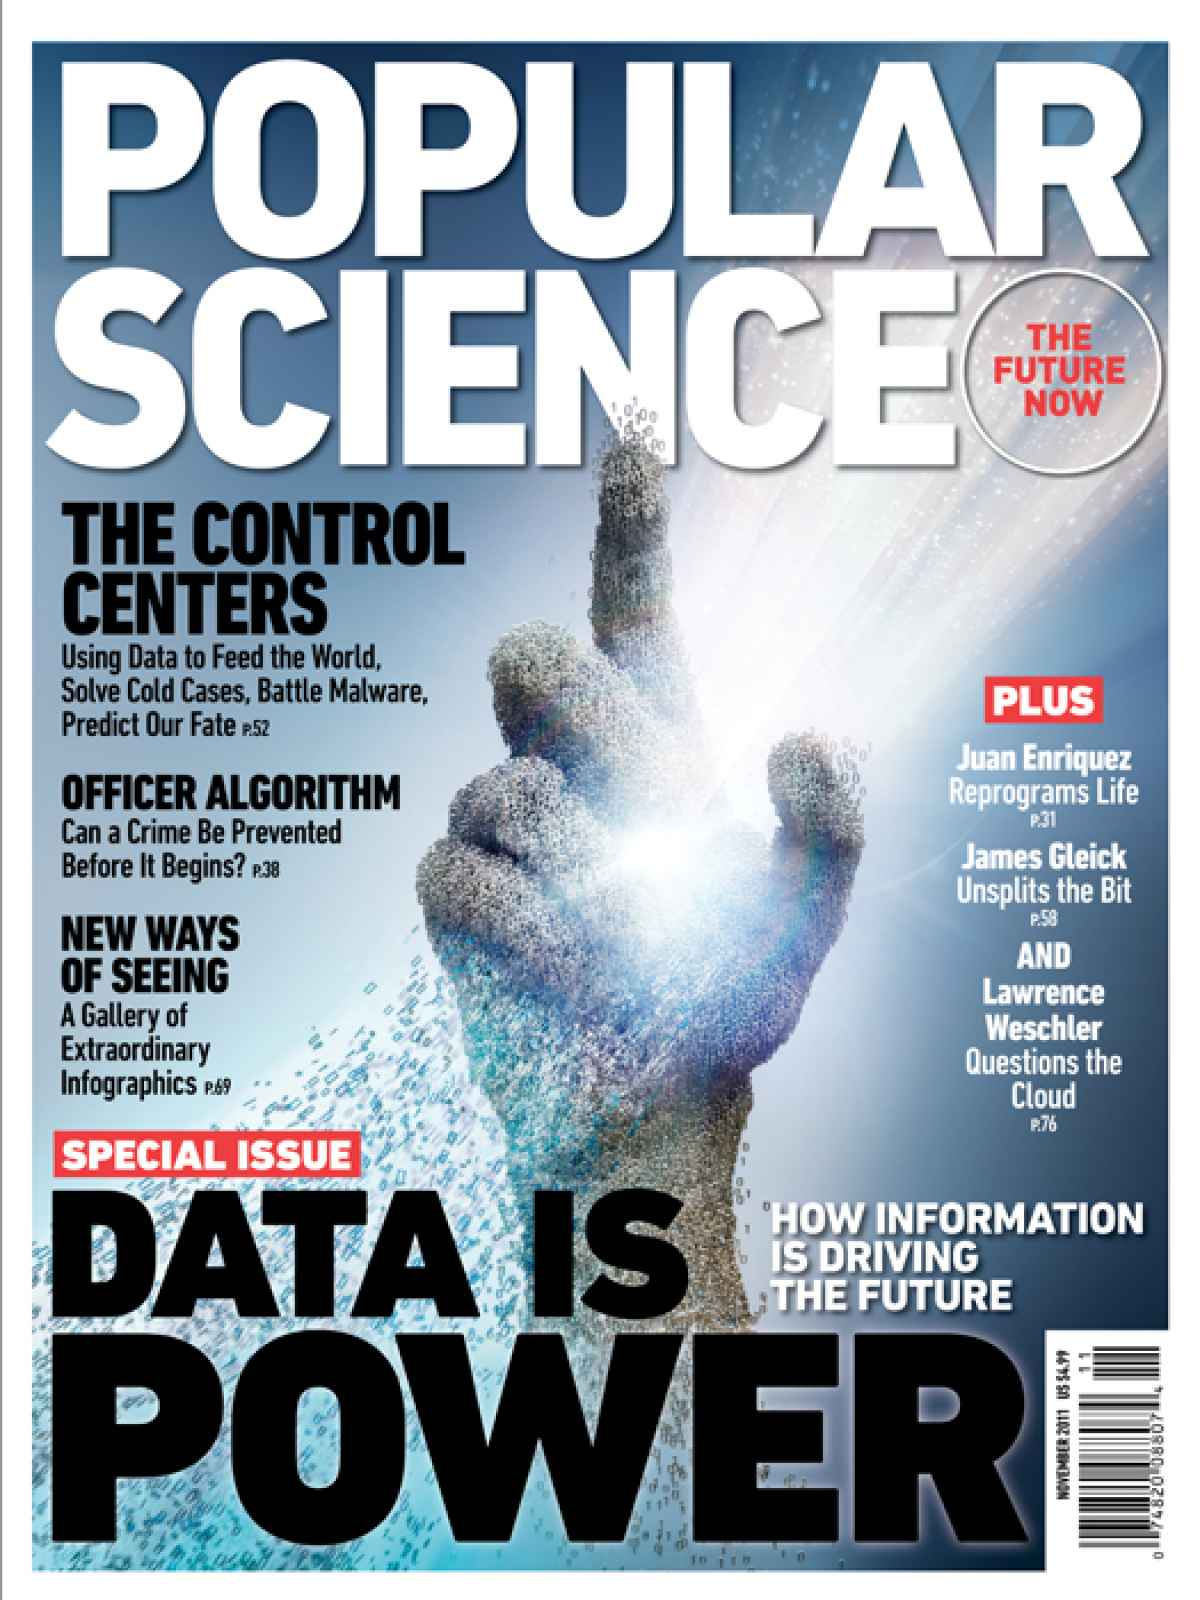
\includegraphics[width=2in]{popular_science}

Data + Mathematical Model -> Better Understanding

\end{frame}

\begin{frame}{Data Reduction in General}

\begin{tikzpicture}

\node(a){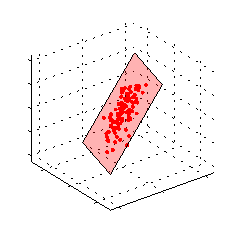
\includegraphics{PCA_3D}};
\node(texta)[below=0cm of a, text width=4.5cm, align=center] {High dimensional data on low-dimensional structure};
\node[right=2cm of a](b){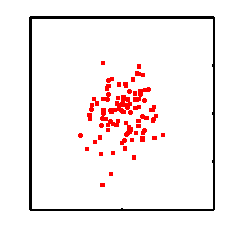
\includegraphics{PCA_2D}};
\node(texba)[below=0cm of b, text width=4cm, align=center] {Reduced dimensionality};
\draw[->] (a) -- (b) node[above, midway]{{\small Data reduction}};
\end{tikzpicture}

Common technique: Principal Component Analysis \\
{\em Project onto hyperplane which captures maximum variance }
\newfootnote{Shlens, ``A Tutorial on Principal Component Analysis}
\end{frame}

\begin{frame}{Diffusion Maps for Nonlinear Data Reduction}
    
    \centering
    \begin{tikzpicture}
        \node (fig1) {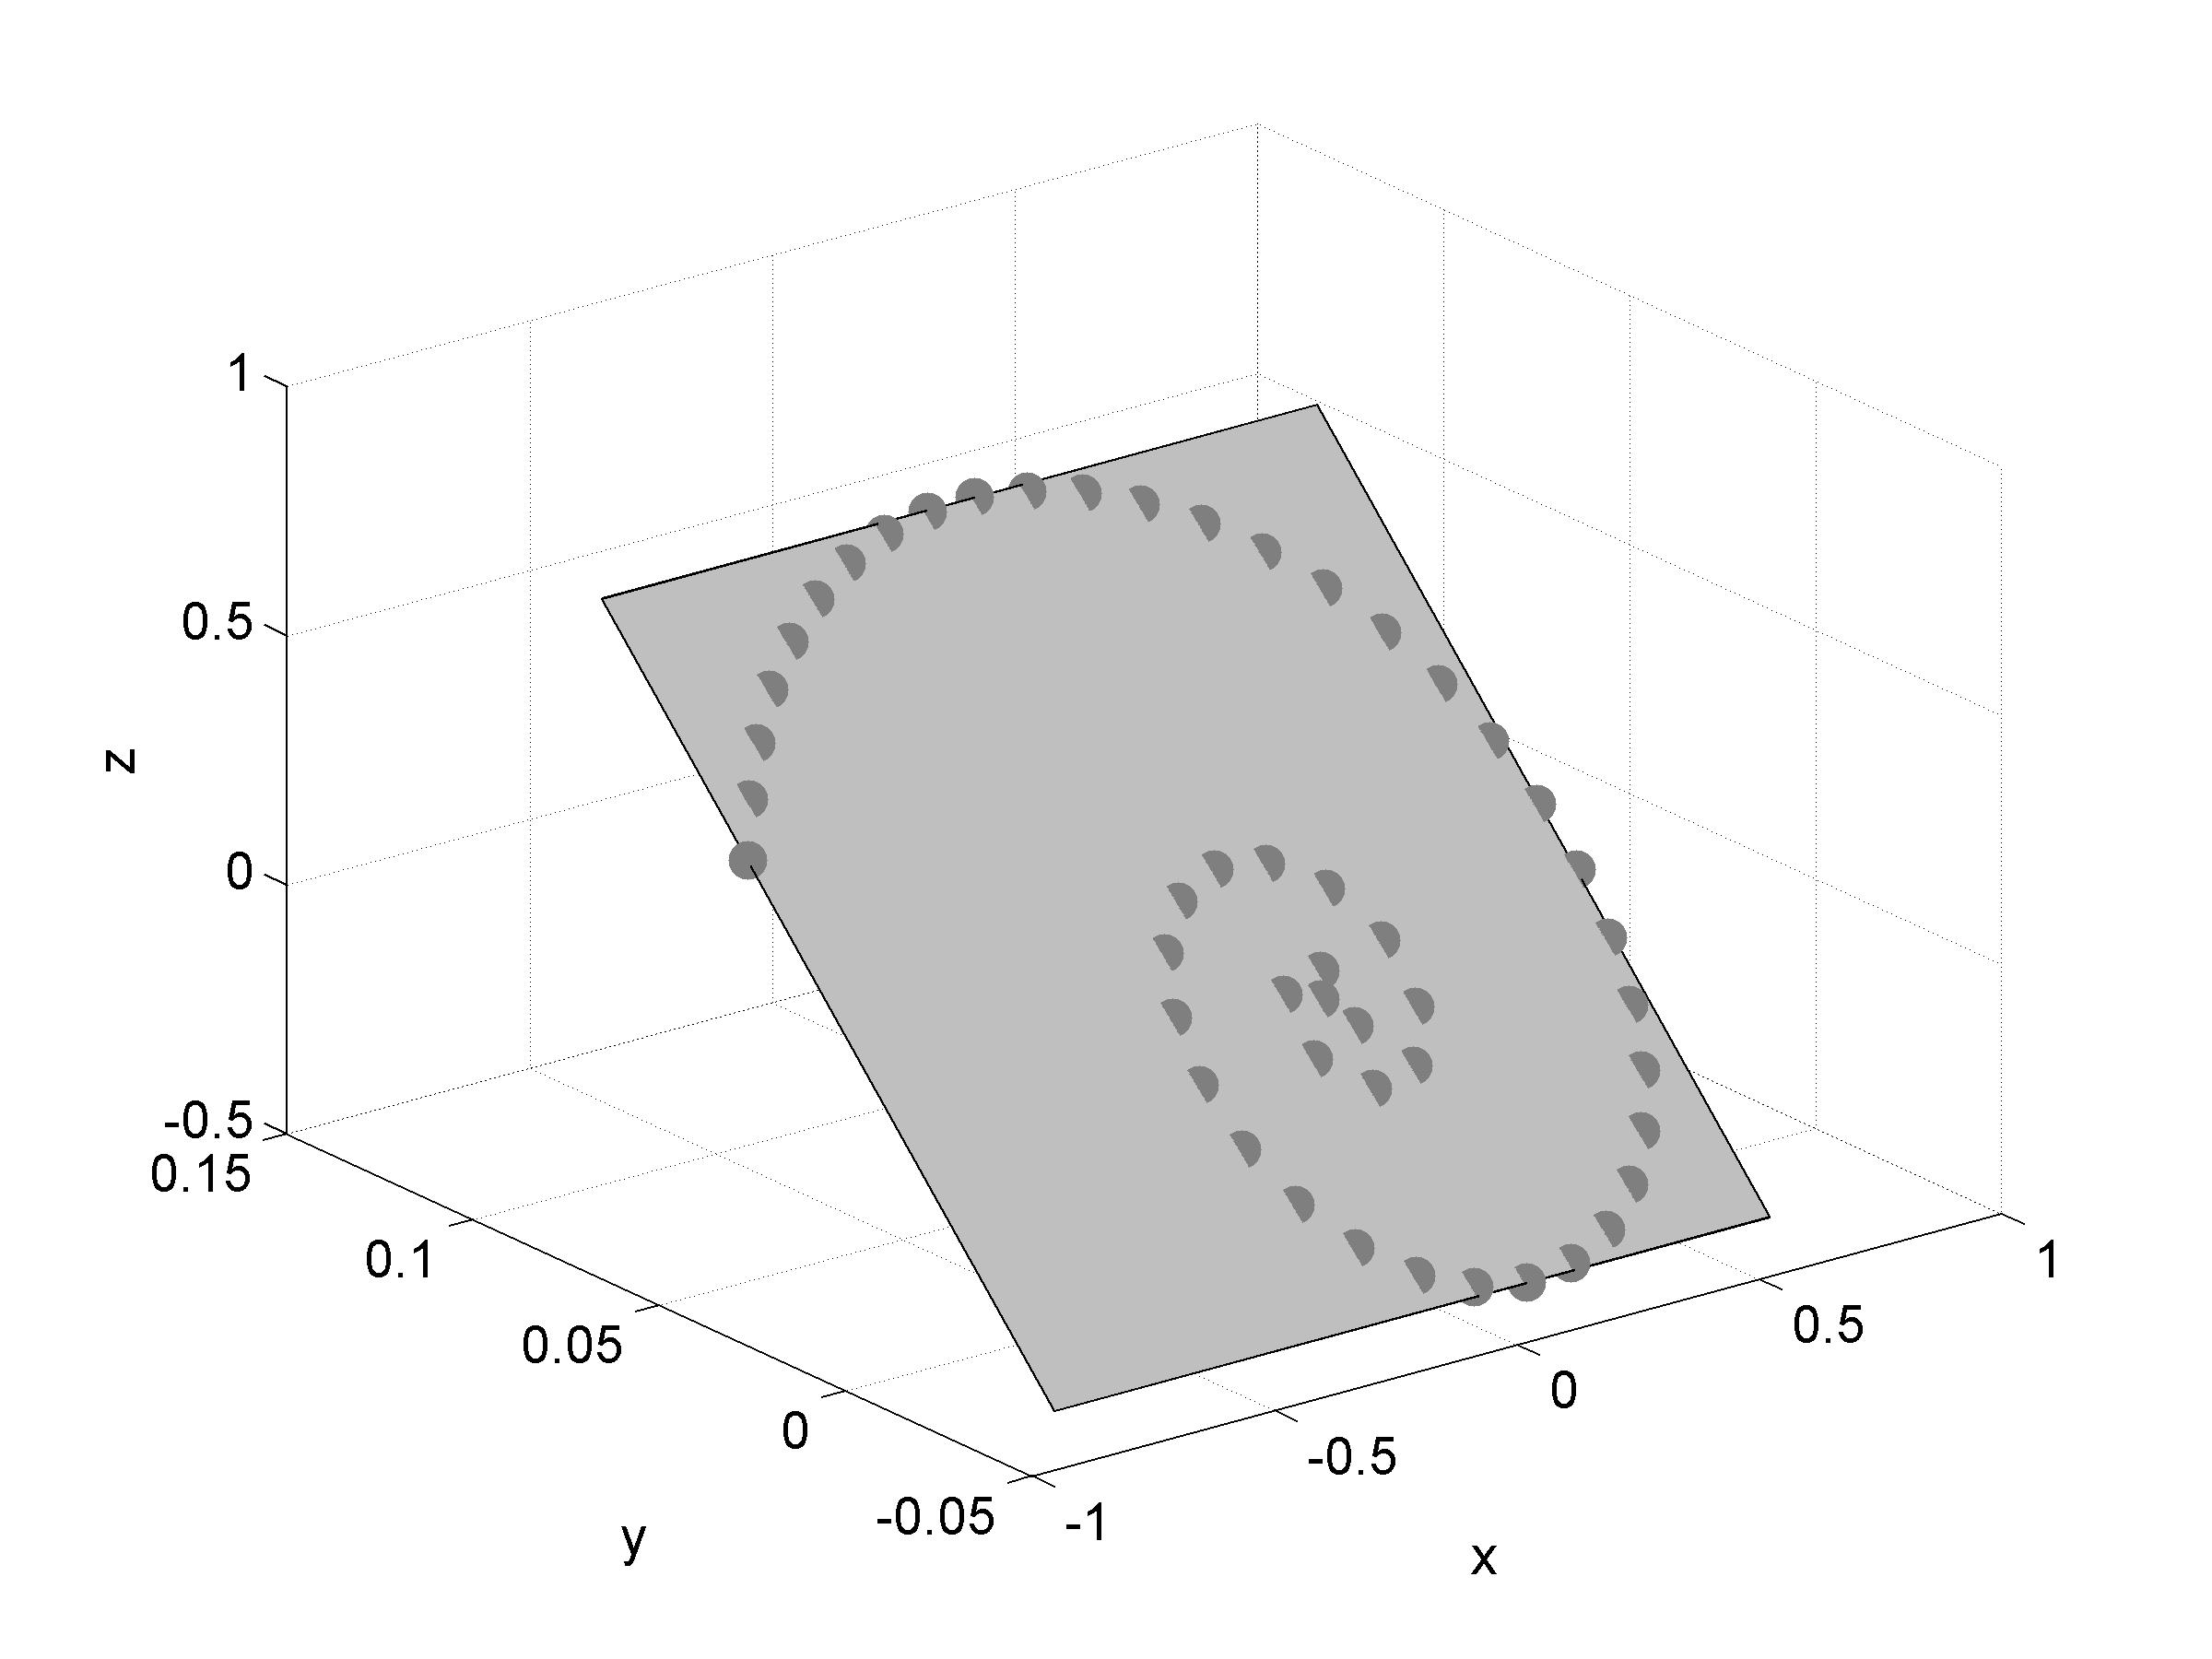
\includegraphics[width=0.4\textwidth]{dmaps_spiral_black_plane_large.jpg}};
        \draw[red,->] (-0.15,-1.2) -- (0.9, -0.9);
        \draw[red,->] (-0.15,-1.2) -- (-1, 0.4);
        \node[right of=fig1, node distance=0.5\textwidth] (fig2) {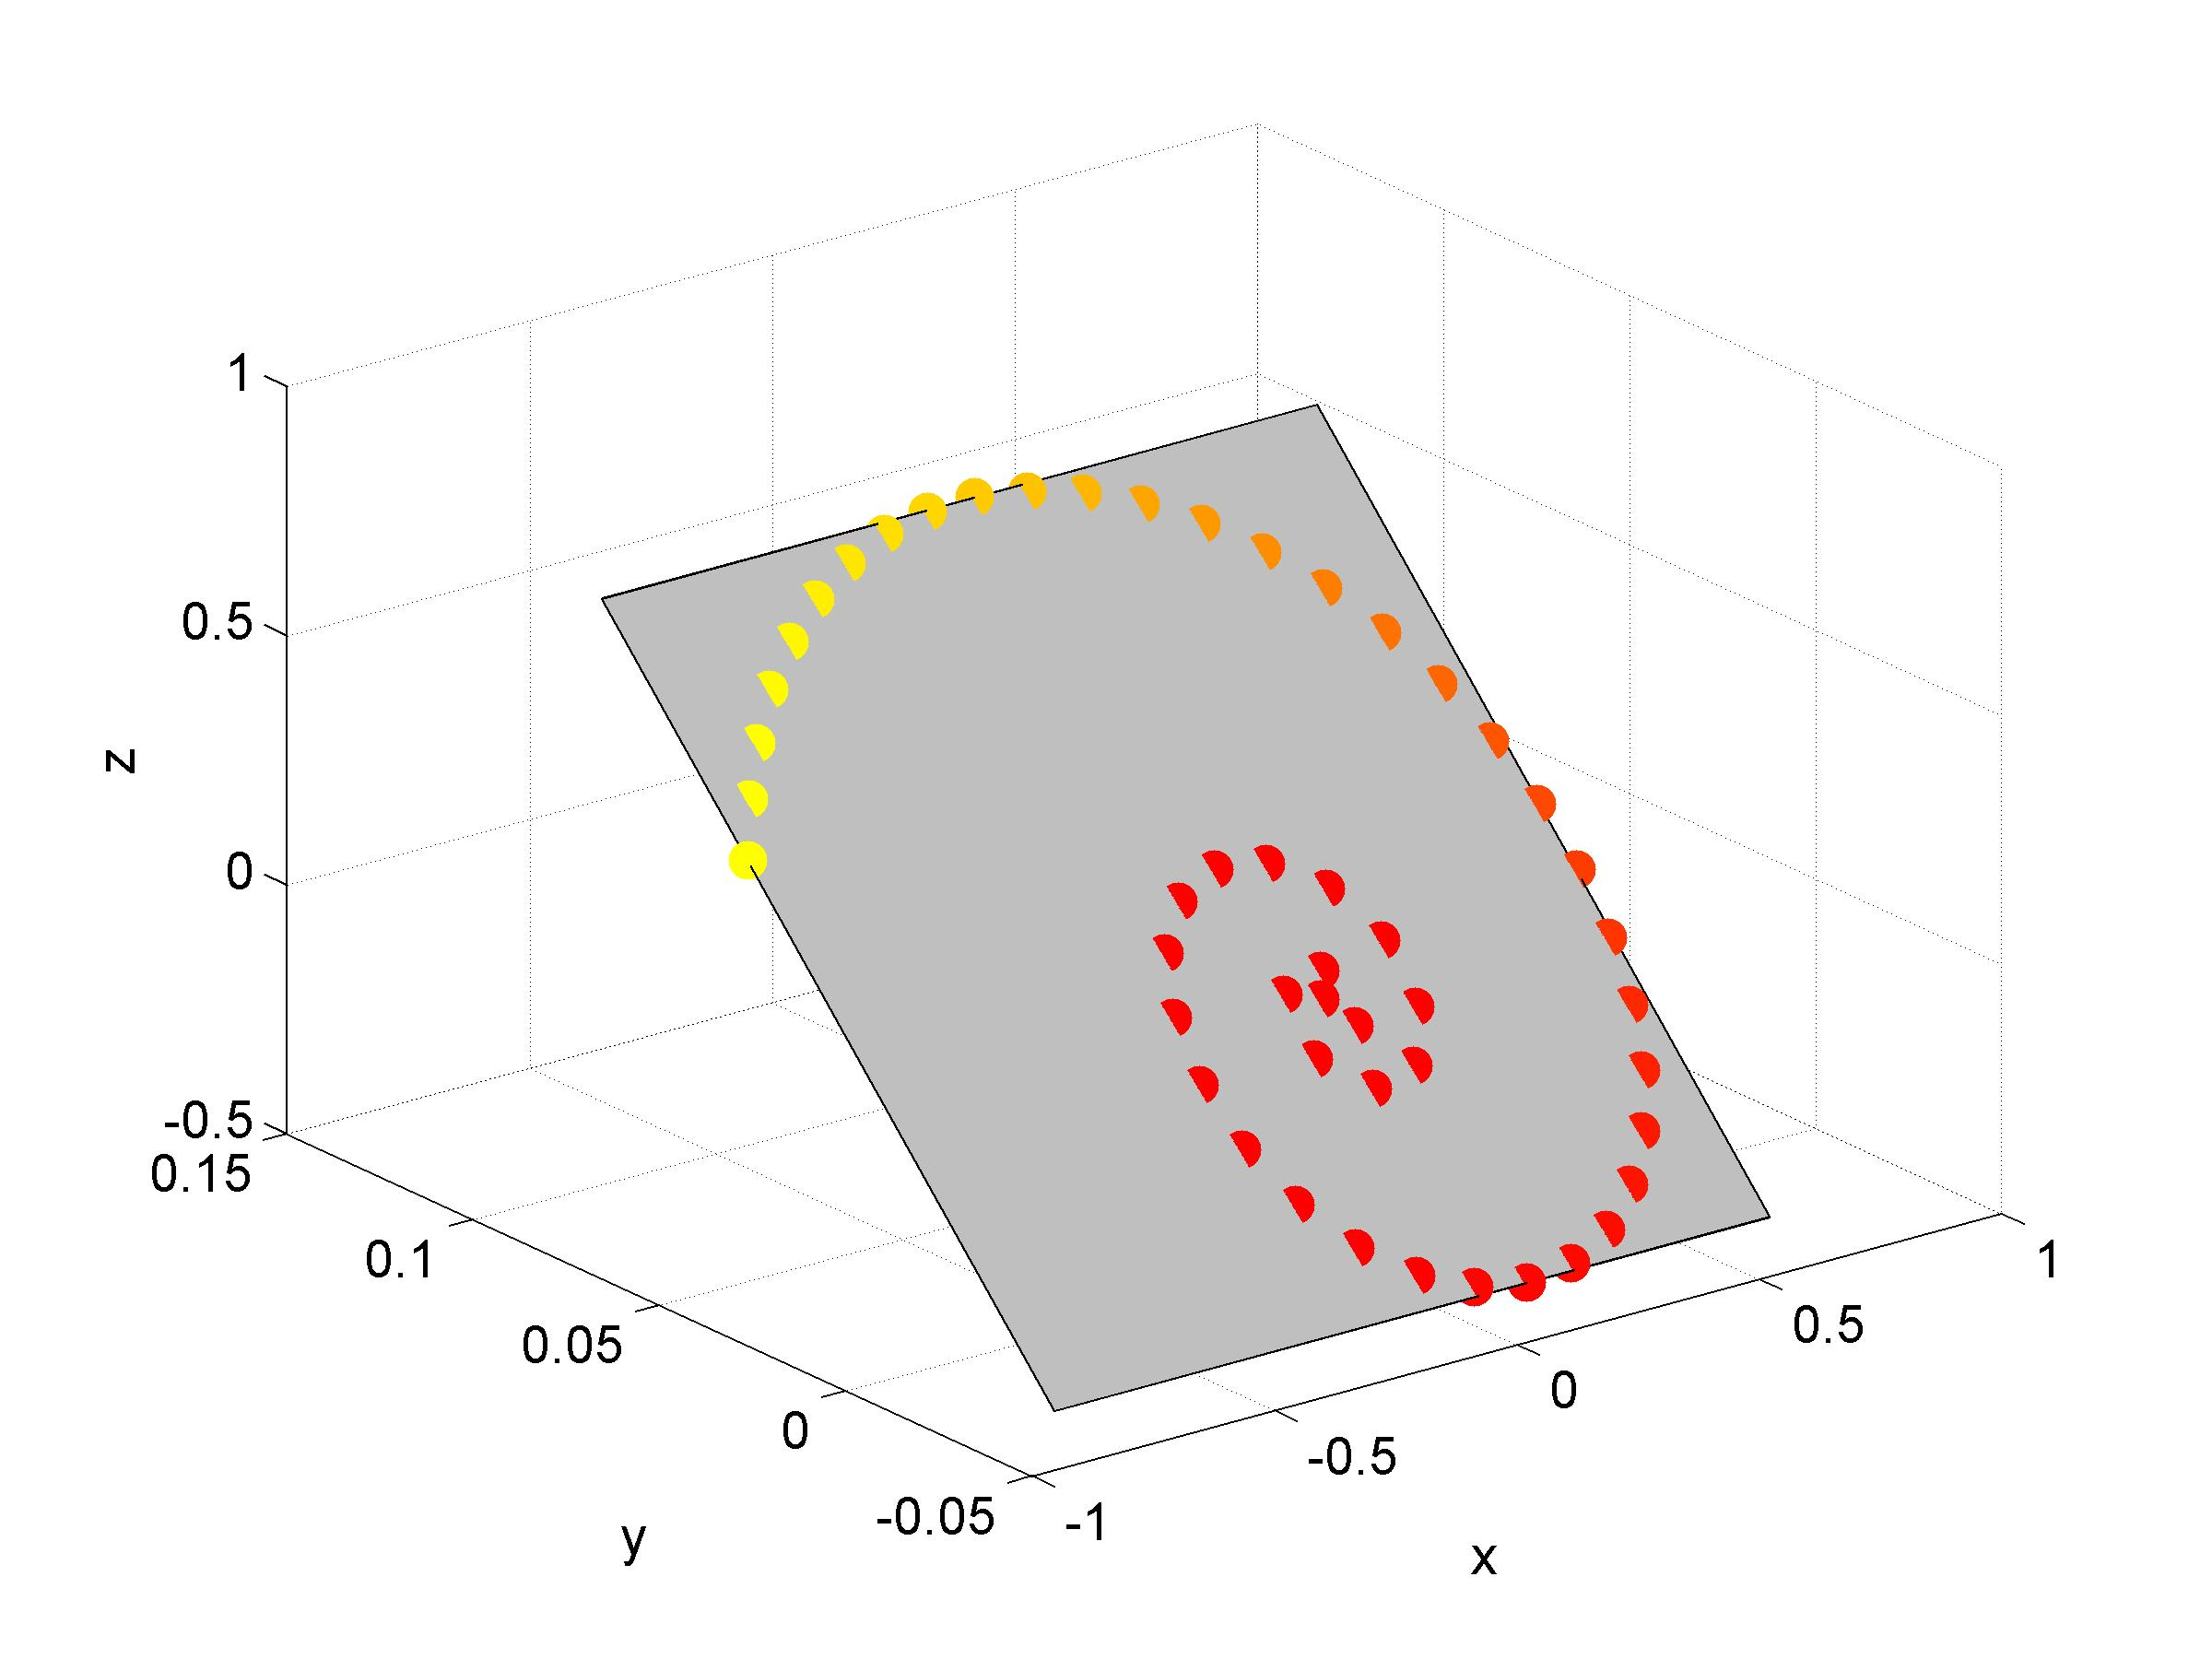
\includegraphics[width=0.4\textwidth]{dmaps_spiral_color_plane_large.jpg}};
        \draw [->] (fig1.east) -- (fig2.west);
        
        \node[below=0cm of fig1, text width=0.4\textwidth, align=center]{Data on a spiral \\ {\scriptsize PCA will find \\two-dimensional plane \par}};
        
        \node[below=0cm of fig2, text width=0.5\textwidth, align=center]{Data colored by first diffusion maps coordinate};
        
    \end{tikzpicture}

	\newfootnote{Coifman {\em et al}, PNAS, 2005.}
 
\end{frame}

\begin{frame}{Eigenfunctions to Parameterize a Manifold}

	\makebox[\textwidth][c]{
	\begin{tikzpicture}[node distance=0cm]
	
	\node(manifold){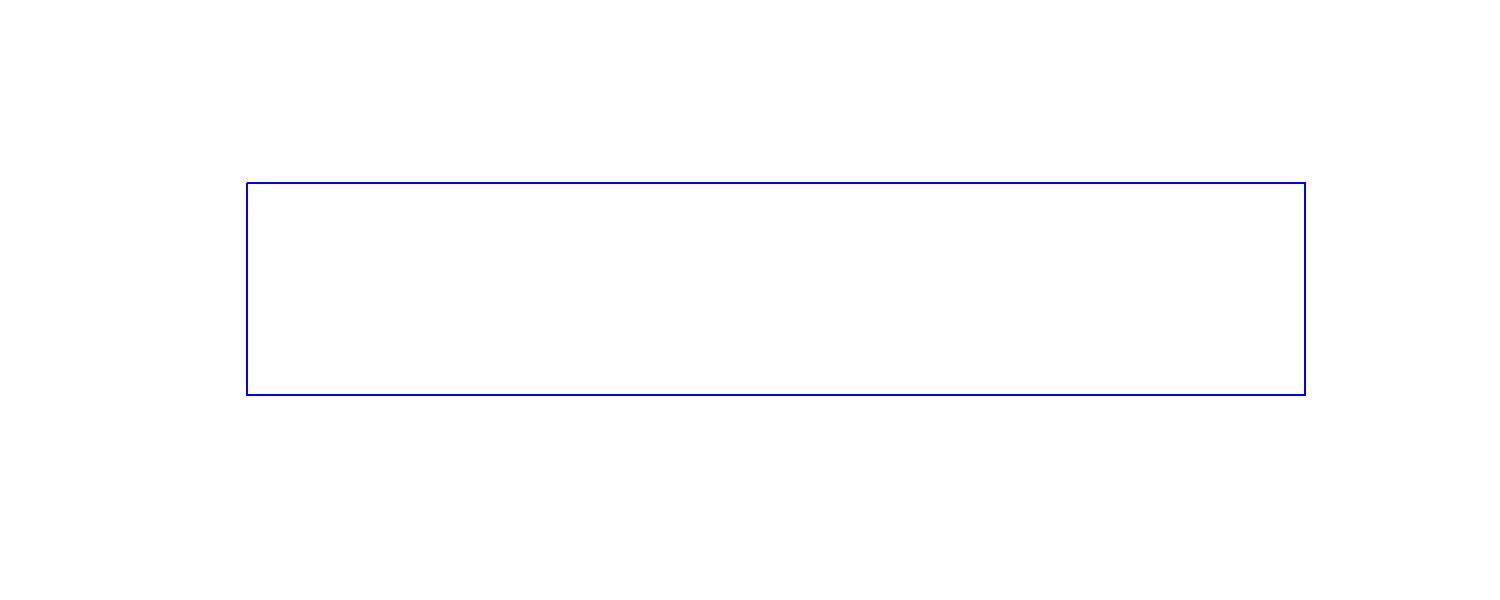
\includegraphics[width=0.3\textwidth]{rect.jpg}};
	\node[above=of manifold, text width=3.5cm, align=center]{{\scriptsize Consider a manifold \par}};
	
	\node[right=of manifold](eigenfunctions){\animategraphics[width=0.35\textwidth]{1}{rect_efunc}{1}{6}};
	\node[above=of eigenfunctions, text width=3.5cm, align=center]{{\scriptsize We want a ``good'' parametrization of~the manifold \par}};
	\node[below=of eigenfunctions, text width=4cm, align=center]{{\scriptsize These parameterizations are the~eigenfunctions of $\nabla^2 \phi$ \par}};
	
	\node[right=of eigenfunctions](eigenvectors){\animategraphics[width=0.35\textwidth]{1}{rect_evec}{1}{6}};
	\node[above=of eigenvectors, text width=3.5cm, align=center]{{\scriptsize Instead, we have data {\em sampled} from the manifold and want to~obtain a parameterization \par}};
	\node[below=of eigenvectors, text width=3.5cm, align=center]{{\scriptsize We therefore {\em approximate} the~Laplacian on the data \par}};

	\end{tikzpicture}
	}

    \vspace{0.1in}

    \centering
    {\small We obtain a similar parametrization for a curved manifold \par}
    \vspace{0.05in}
    
\includegraphics[width=0.18\textwidth]{circle.jpg}
    \hspace{0.03\textwidth}
    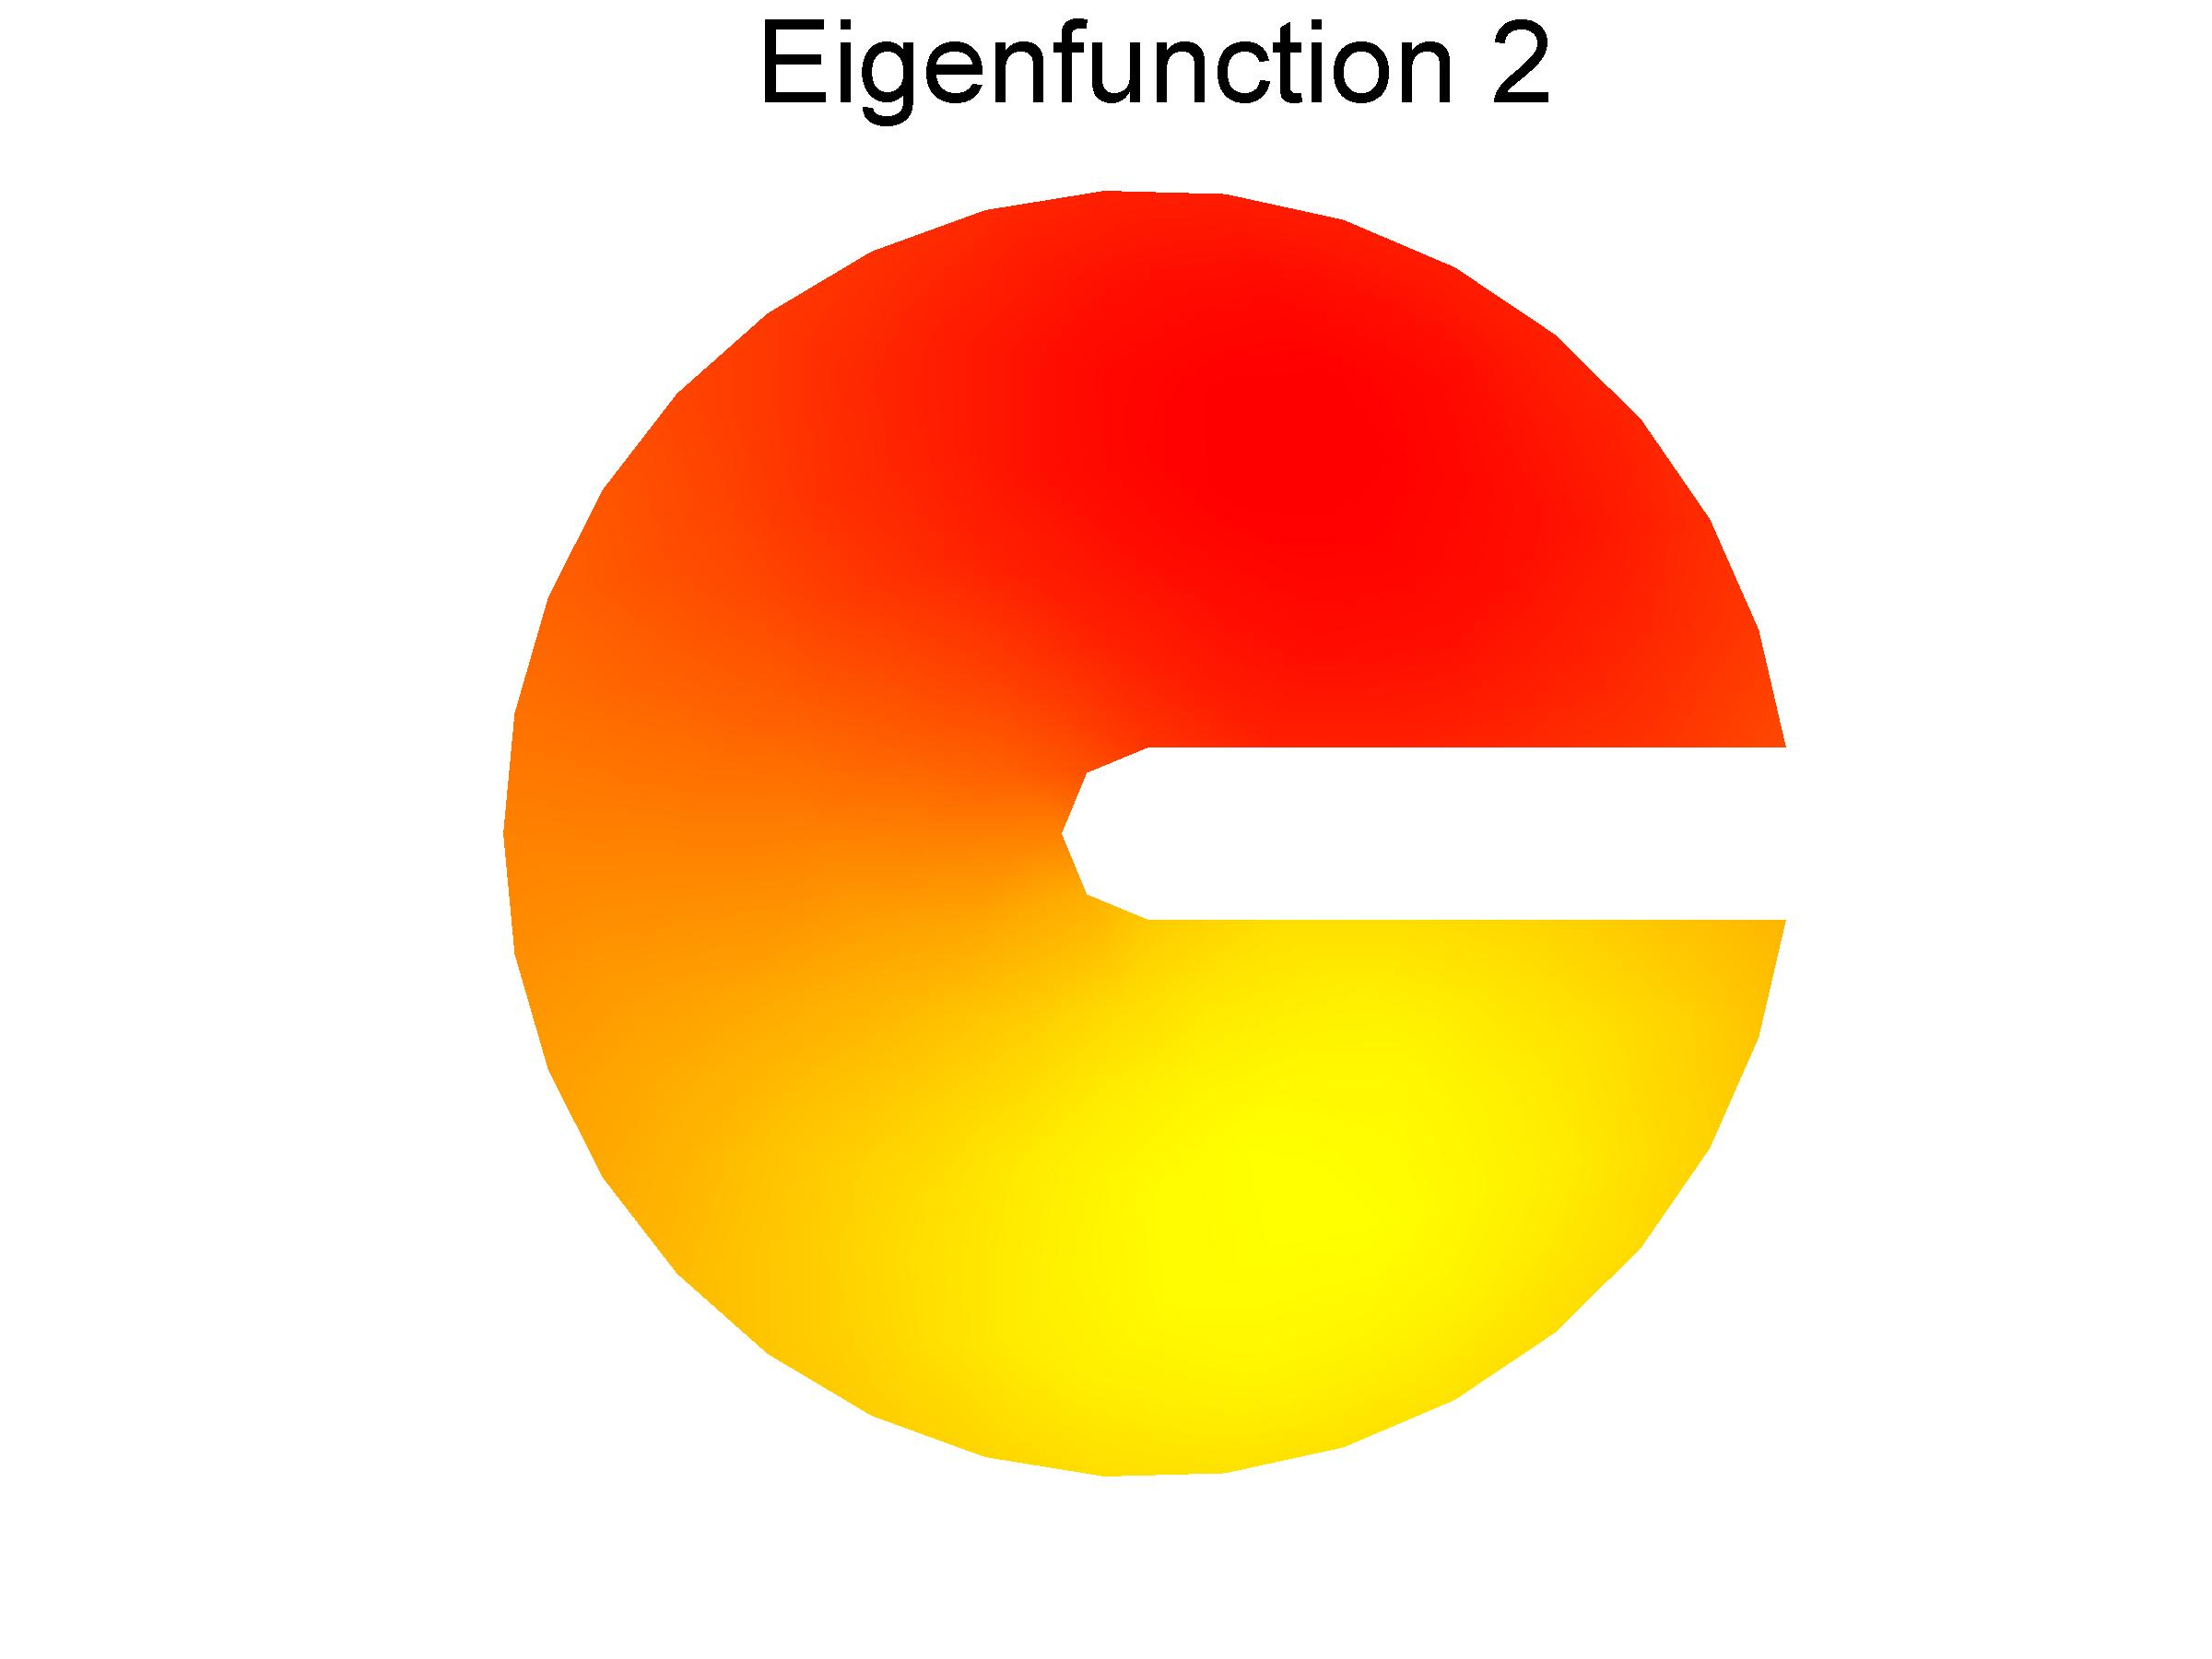
\includegraphics[width=0.18\textwidth]{circle_efunc1.jpg}
    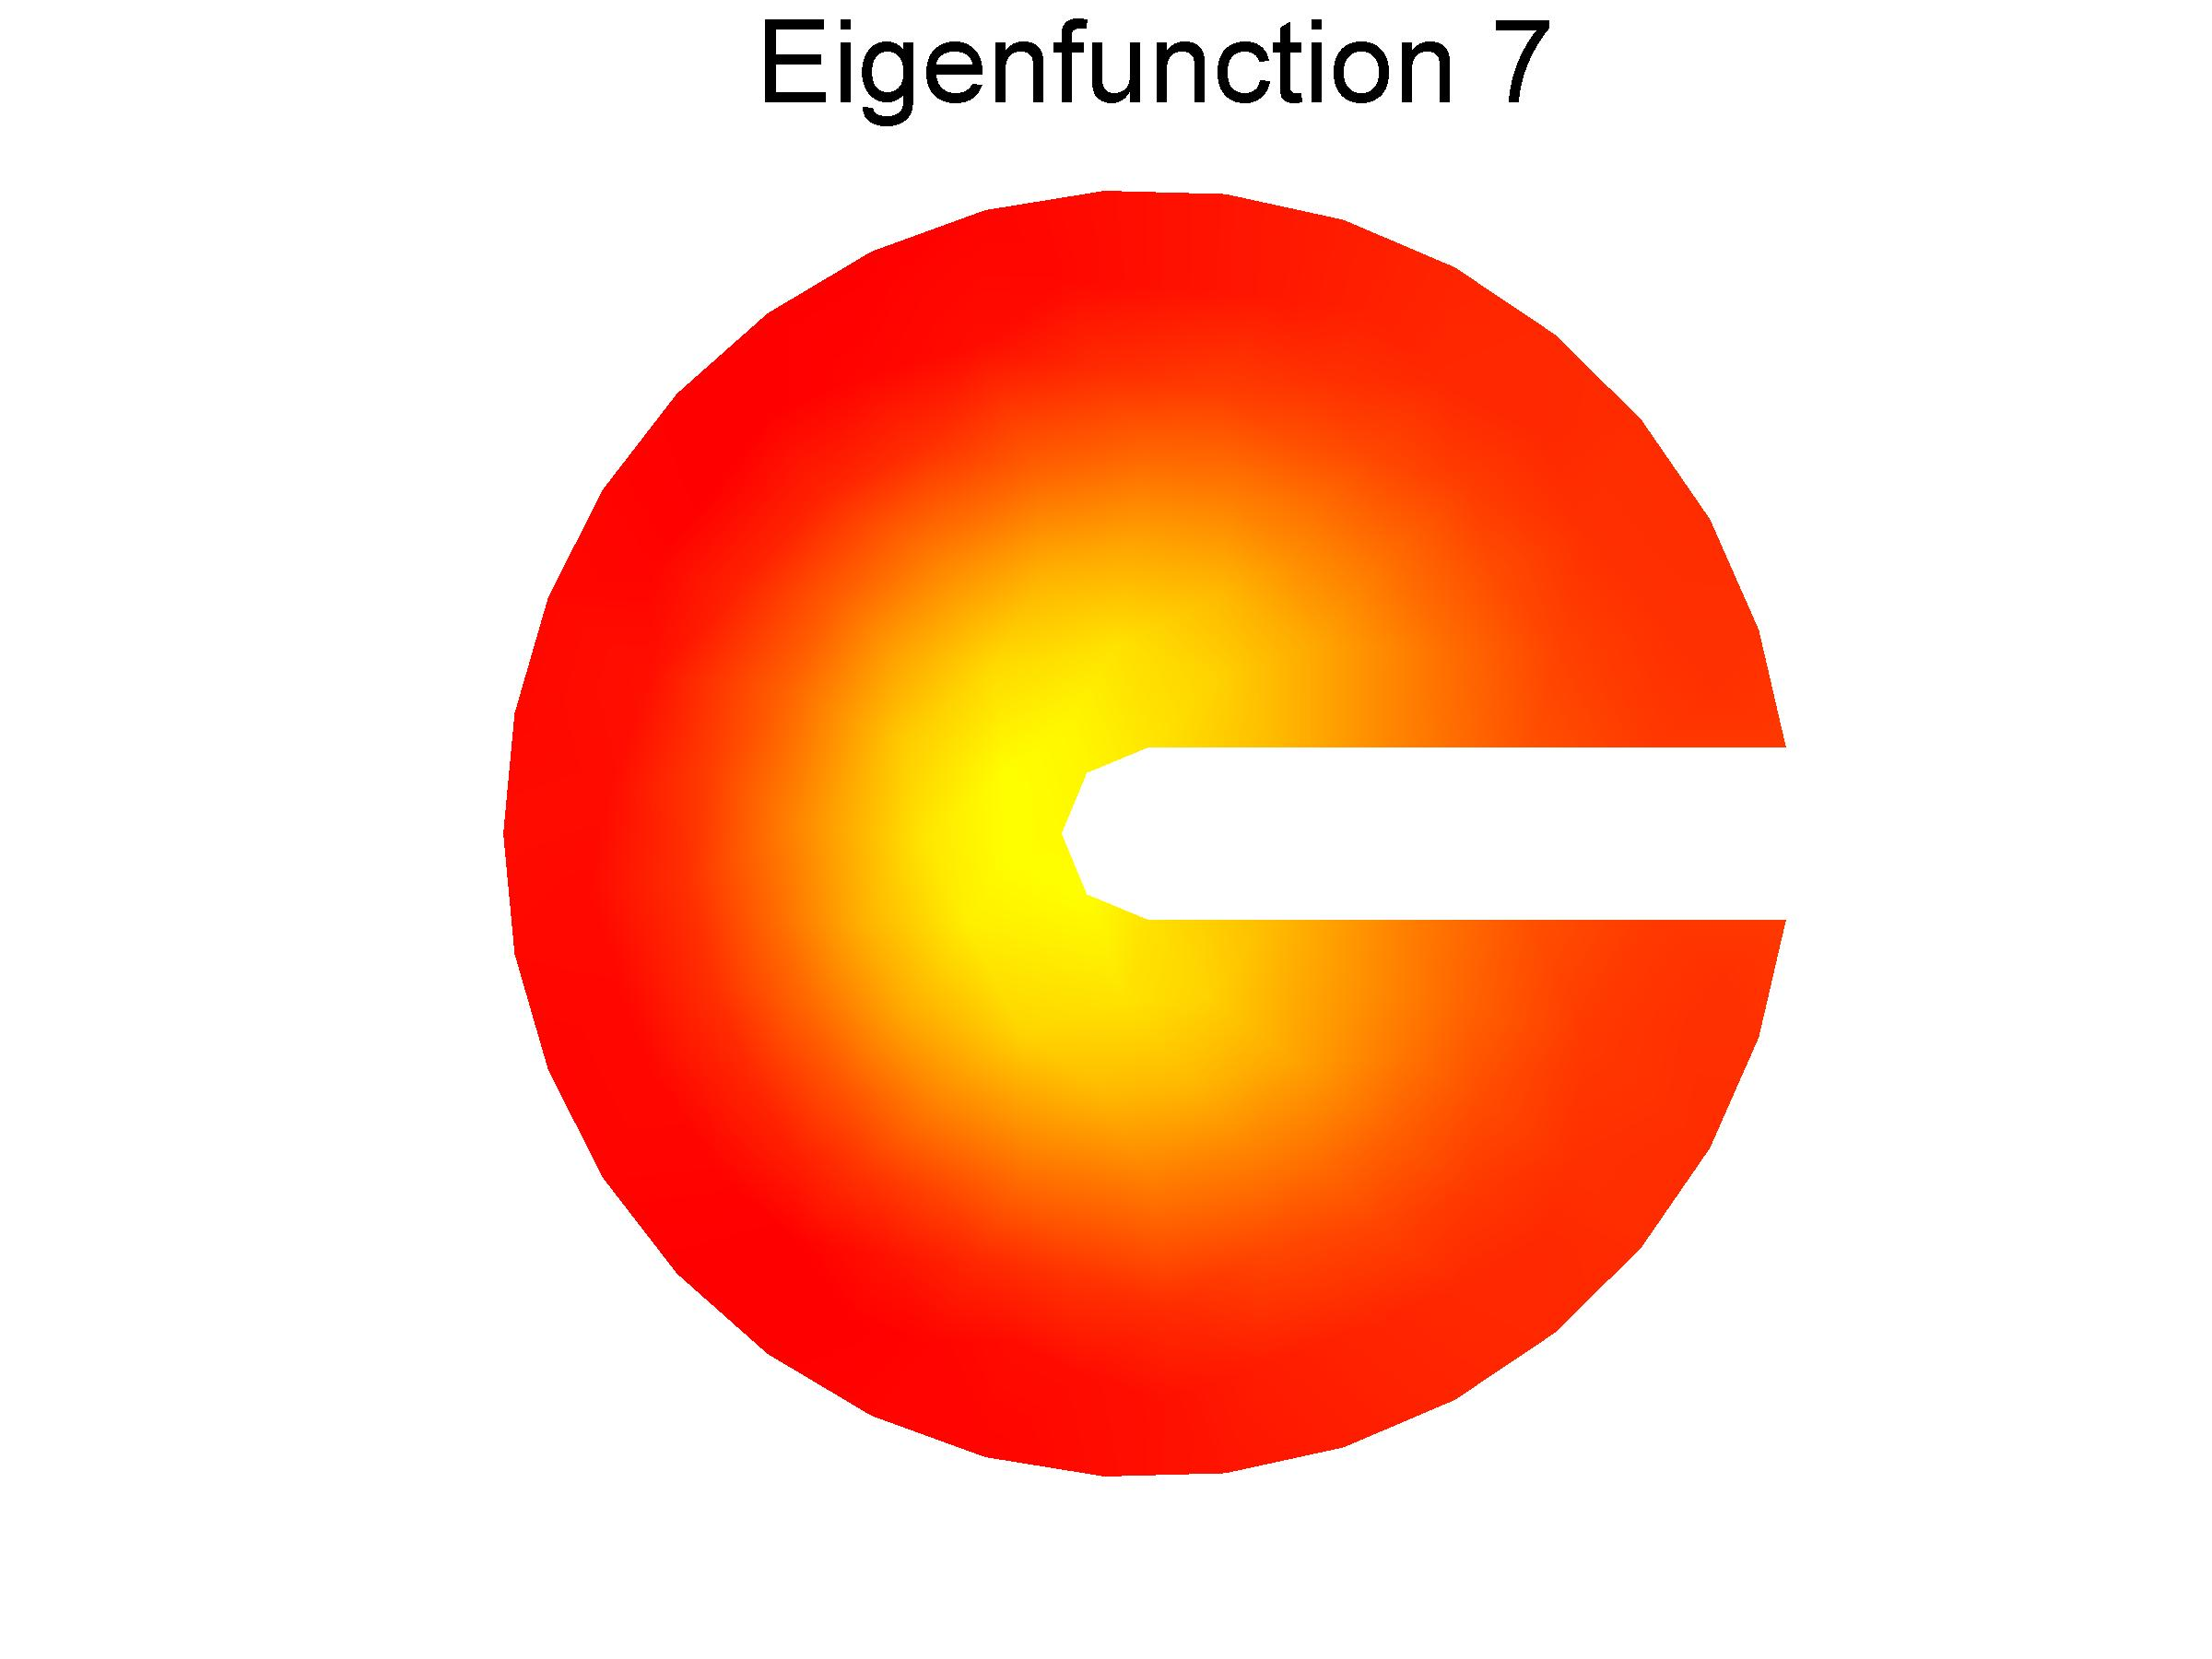
\includegraphics[width=0.18\textwidth]{circle_efunc6.jpg}
    \hspace{0.03\textwidth}
    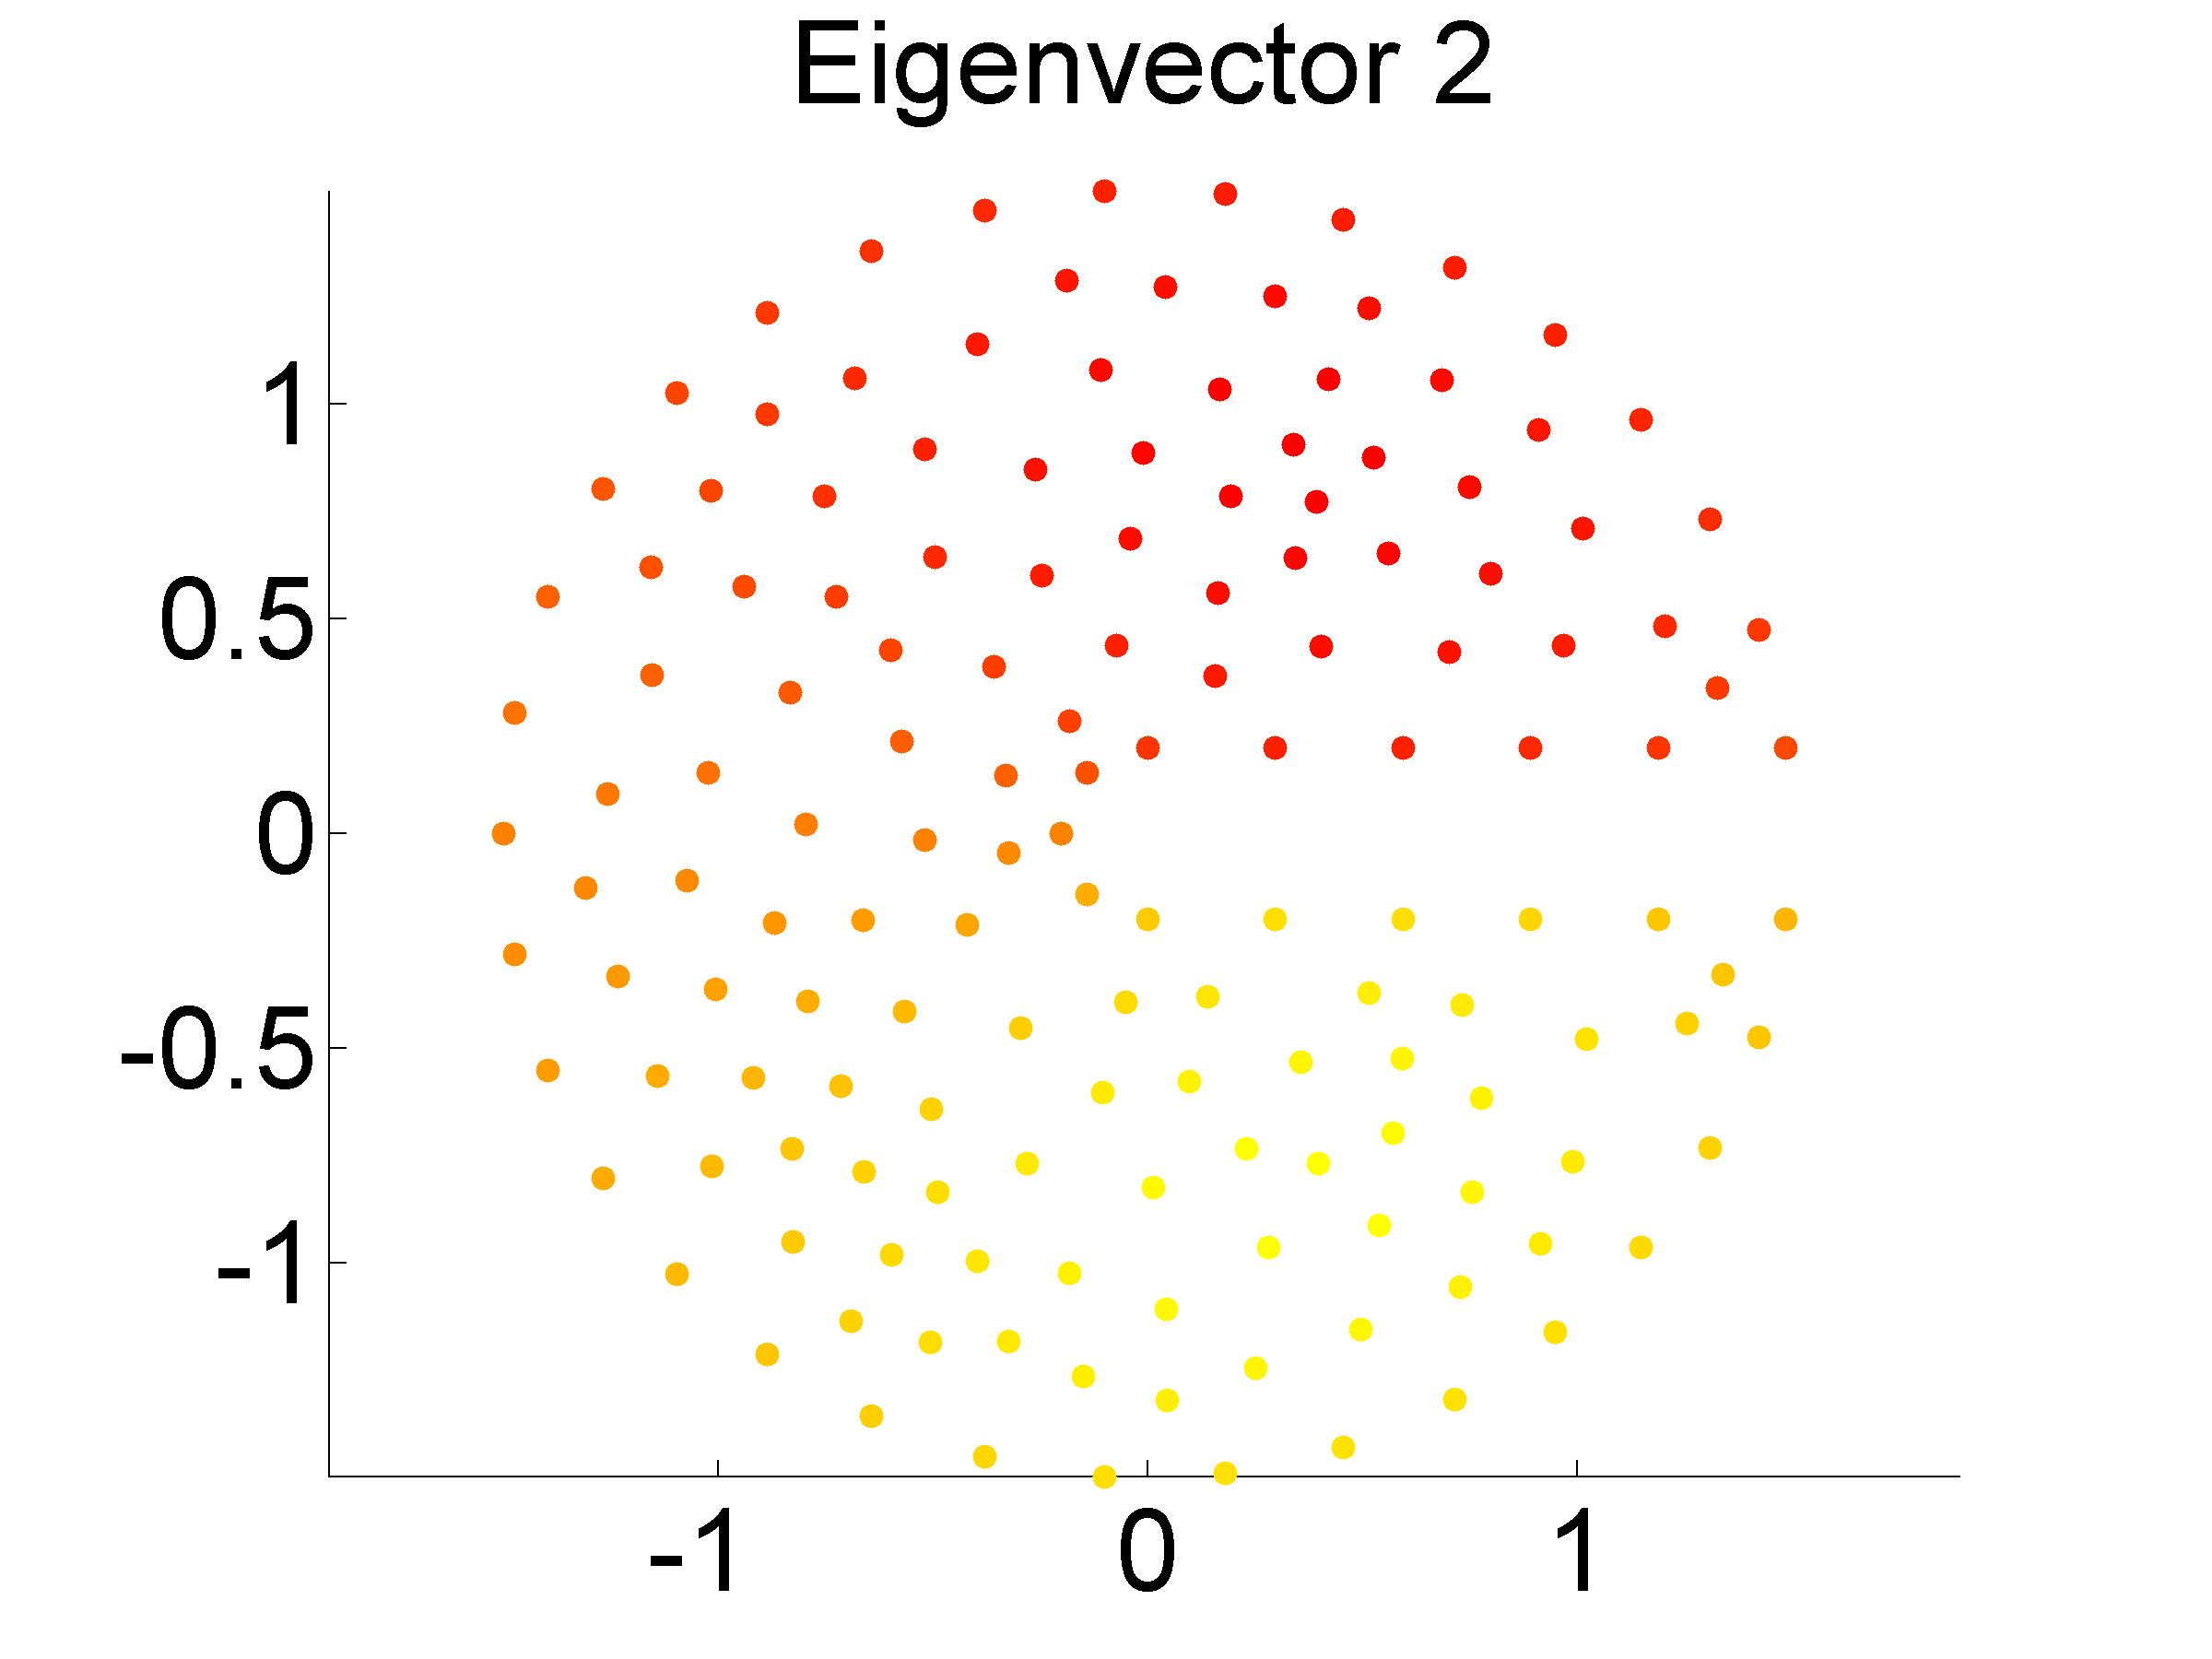
\includegraphics[width=0.18\textwidth]{circle_evec1.jpg}
    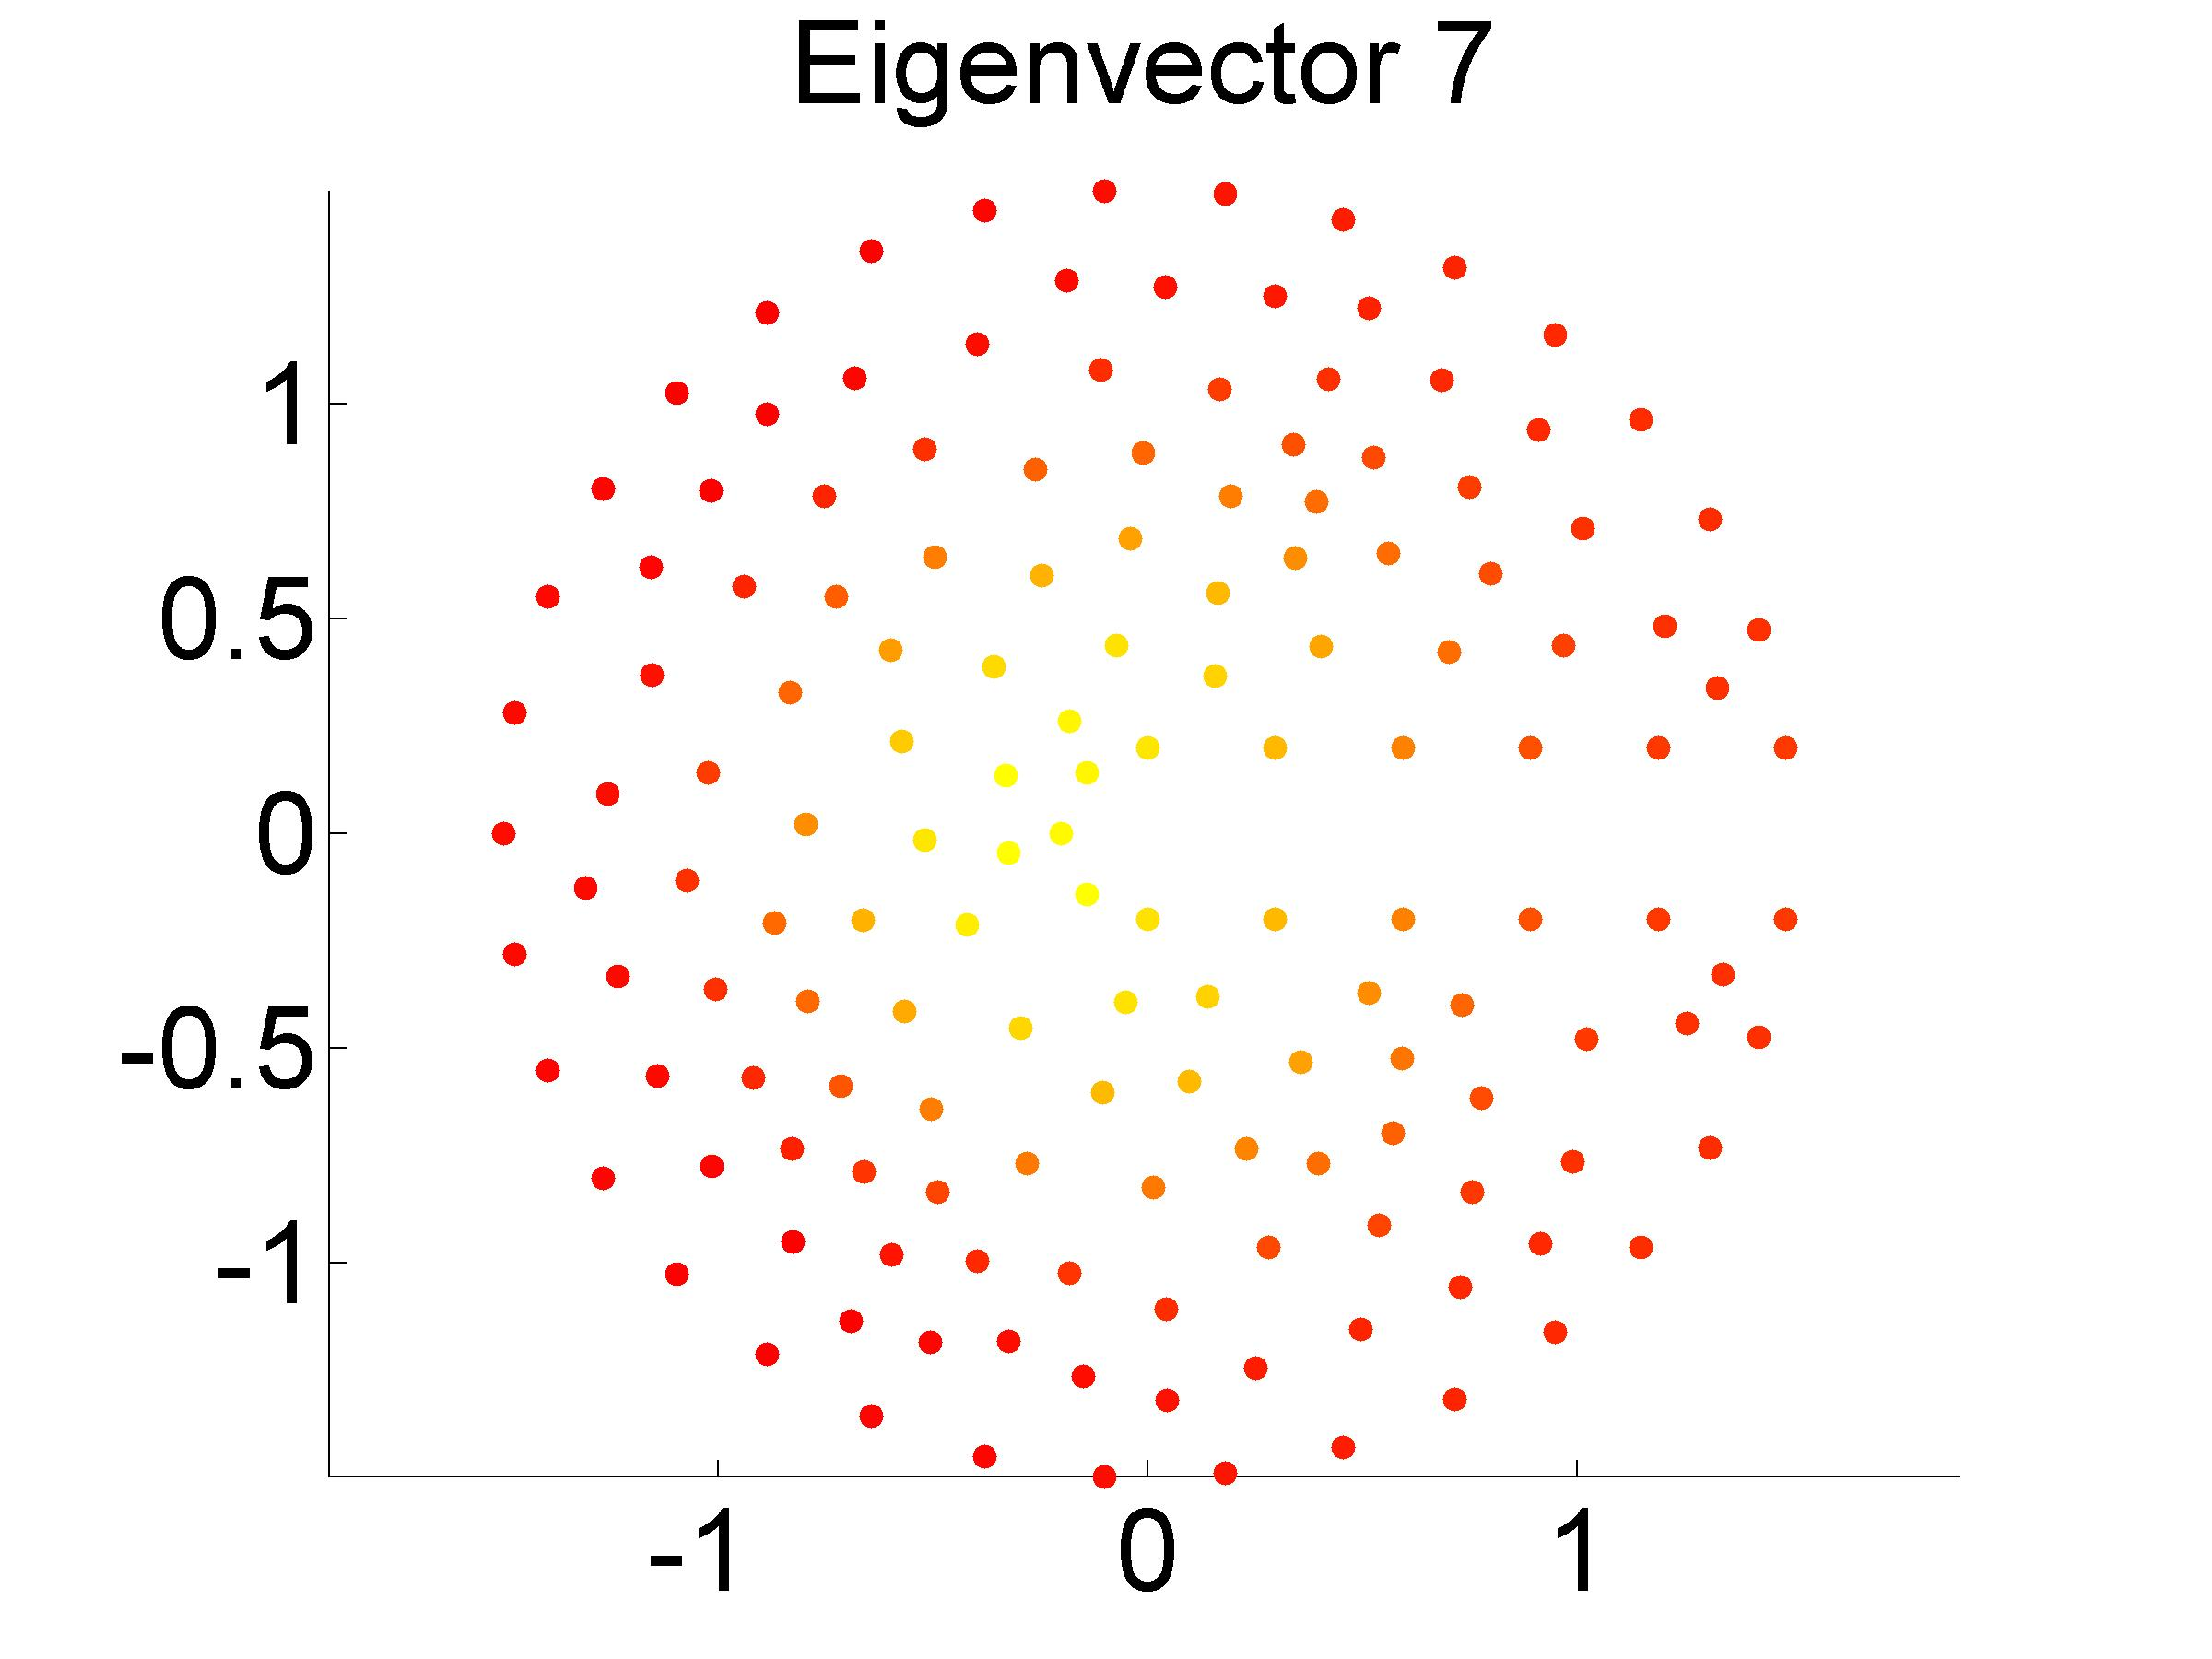
\includegraphics[width=0.18\textwidth]{circle_evec6.jpg}\\

    \vspace{0.05in}

    {\small Diffusion maps approximates the eigenfunctions for a manifold \\ using data sampled from the manifold \par}

\end{frame}

\begin{frame}{Diffusion Maps Implementation }

	
	\newfootnote{Coifman {\em et al}, PNAS, 2005}
	
	\makebox[\textwidth][c]{

	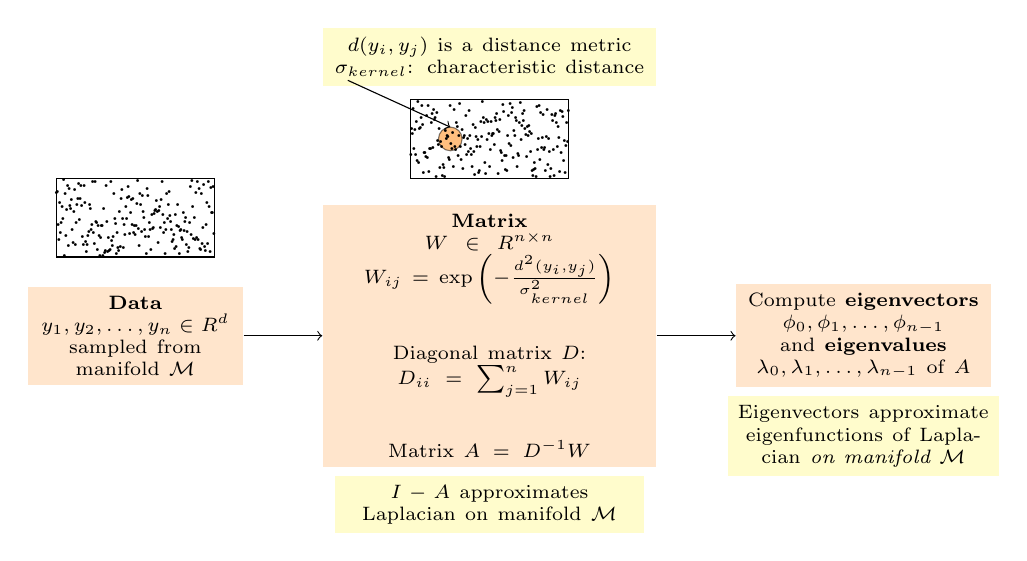
\begin{tikzpicture}
	
	\node[fill=orange!20, text width=2.5cm, align=center](data){{\scriptsize {\bf Data} $y_1, y_2, \dots, y_n \in \mathbb{R}^d$  sampled from manifold $\mathcal{M}$ \par}};
	
	\draw (-1,1) rectangle (1,2);
	\foreach \i in {-100,...,100}
	{
	 	\draw (\i/100,0.48*rand+1.35) node[anchor=south] {.};
	}

	\node[fill=orange!20, text width=4cm, right=of data, align=center](matrix){{\scriptsize {\bf Matrix} \\
        $ W  \in \mathbb{R}^{n \times n} $ \\
        $W_{ij} = \exp \left( -\frac{d^2 (y_i, y_j)}{\sigma_{kernel}^2}  \right)  $ \\
        \vspace{0.5cm}
	 Diagonal matrix $D$: \\
	 $D_{ii} = \sum_{j=1}^{n} W_{ij}$\\ 
	 \vspace{0.5cm}
	 Matrix $A =  D^{-1} W$ \par}};
	
	\node[fill=orange!20, text width=3cm, right=of matrix, align=center](eigenvectors){{\scriptsize Compute {\bf eigenvectors} $\phi_0, \phi_1, \dots, \phi_{n-1}$ and {\bf eigenvalues} $\lambda_0, \lambda_1, \dots, \lambda_{n-1}$ of $A$ \par}};

		\node[fill=yellow!20, text width=4cm, above=1.5cm of matrix, align=center](distance){{\scriptsize $d(y_i, y_j)$ is a distance metric \\
		$\sigma_{kernel}$: characteristic distance \par}};

	\draw (3.5,2) rectangle (5.5,3);
	\draw[fill=orange, opacity=0.5] (4,2.5) circle (0.15);
	
	\draw[->] (distance) ++ (-1.8,-0.3) -- (4,2.65);
	
	\foreach \i in {-100,...,100}
	{
	 	\draw (\i/100+4.5,0.48*rand+2.35) node[anchor=south] {.};
	}
		\node[fill=yellow!20, text width=3.7cm, below=0.1cm of matrix, align=center](laplacian){{\scriptsize $I-A$ approximates Laplacian on manifold $\mathcal{M}$ \par}};
		
		\node[fill=yellow!20, text width=3.2cm, below=0.1cm of eigenvectors, align=center](eigenfunctions){{\scriptsize Eigenvectors approximate eigenfunctions of Laplacian {\em on~manifold} $\mathcal{M}$ \par}};
		
		\draw[->] (data.east) -- (matrix.west);
		\draw[->] (matrix.east) -- (eigenvectors.west);
		%\draw[->] (matrix.south) -- (laplacian.north);
		%\draw[->] (eigenvectors.south) -- (eigenfunctions.north);
		

	\end{tikzpicture}
	}
	

\end{frame}

\begin{frame}{Data and Dynamics}

Many systems of engineering interest involve {\em dynamics}

gene expression

fluid flow

chemical reactions


Advances in simulations and experiments means there is more data available for these systems



\end{frame}

\begin{frame}{Focus of Thesis}

Adapting {\bf data mining algorithms} for the analysis of data from {\bf dynamical systems}

\section{Multiscale Data}

\begin{itemize}

\item Multiscale data

\item Imaging data

\item Detecting changes in dimensionality

\end{itemize}

\end{frame}


\begin{frame}{Motivation}

\centering
Multiscale time series are ubiquitous

\begin{tikzpicture}

\node(stockmarket){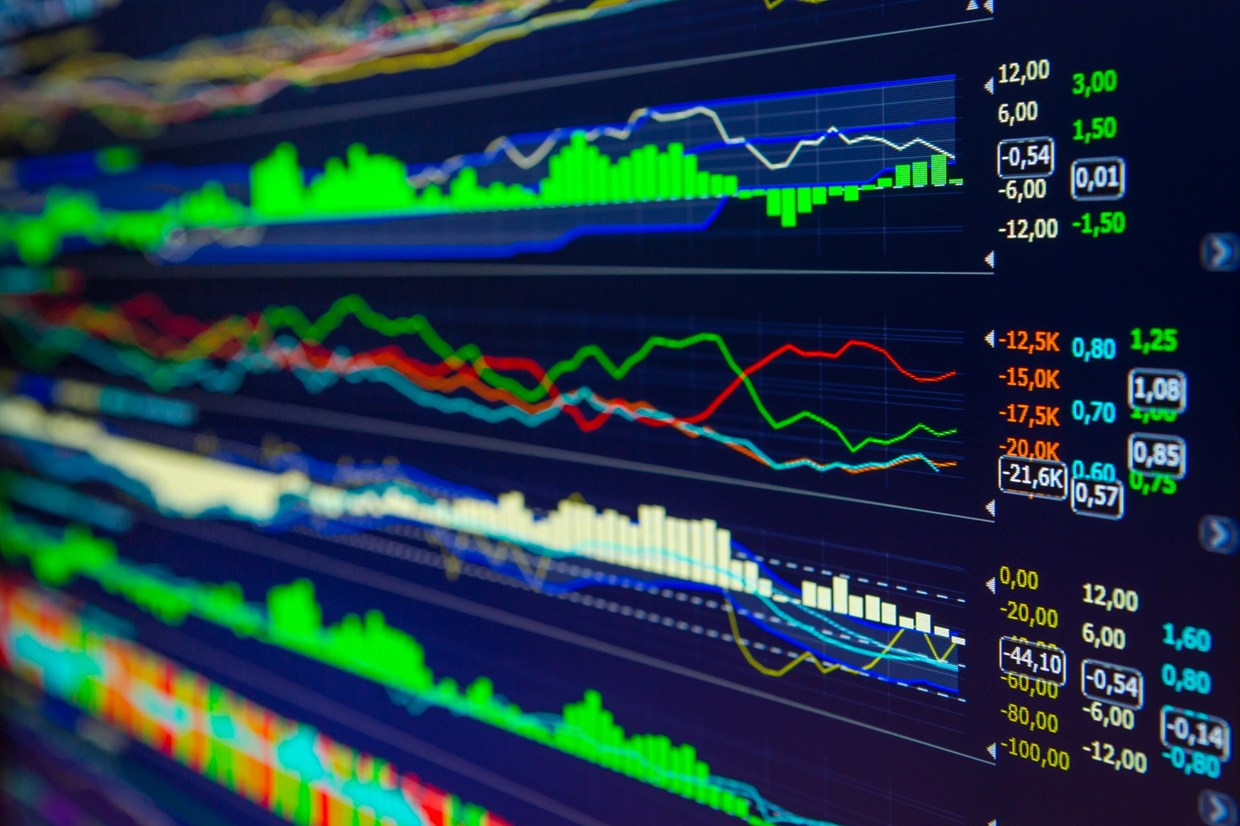
\includegraphics[width=1in]{stockmarket}};
\node[below=0cm of stockmarket, align=center, text width=1.2in]{{\scriptsize Financial data \par} };

\node[left=of stockmarket](proteins){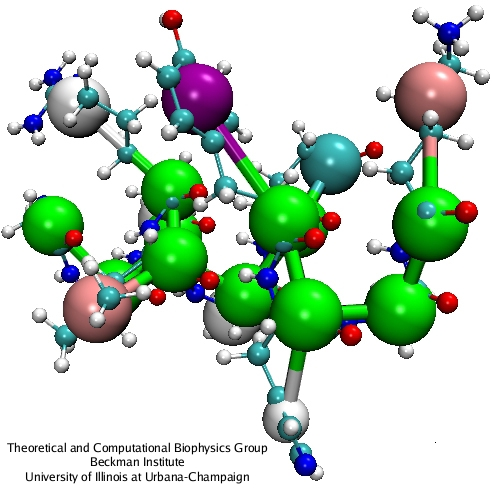
\includegraphics[width=1in]{protein_CG}};
\node[below=0cm of proteins, align=center, text width=1.2in]{{\scriptsize Molecular simulations \par} };
%\node[below=0cm of DNA, align=center, text width=1.2in](DNA_text){DNA replication \\ {\scriptsize Audit {\em et al}, {\em Nature Protocols}, 2013 \par}};

\node[left=of proteins](rxnnetwork){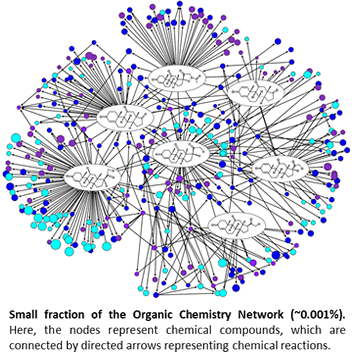
\includegraphics[width=1in]{rxn_networks}};
\node[below=0cm of rxnnetwork, align=center, text width=1in]{{\scriptsize Chemical reaction networks \par} };

\end{tikzpicture}

\newfootnote{{\tiny \texttt{ www.nercenergy.com/research/chemical\_networks.html; www.ks.uiuc.edu/Research/CG; www.wired.co.uk/news/archive/2013-05/8/wikipedia-views-stock-market }}}

\vspace{0.5cm}

\centering
Want to extract the {\em slow variables} \\that govern the system dynamics

\end{frame}


\begin{frame}{How to Reduce?}

\begin{block}{Model reduction}

\centering
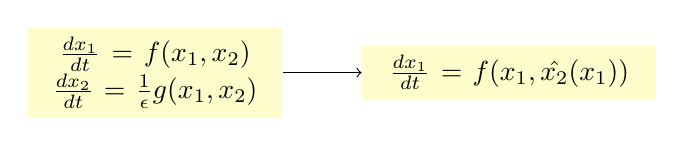
\begin{tikzpicture}
\node[fill=yellow!20, text width=3cm, align=center](a) {$ \frac{dx_1}{dt} = f(x_1,x_2) $ $ \frac{dx_2}{dt} = \frac{1}{\epsilon} g(x_1,x_2)$};
\node[right=of a,fill=yellow!20, text width=3.5cm, align=center](b) {$ \frac{dx_1}{dt} = f(x_1,\hat{x_2}(x_1)) $};

\draw[->] (a) -- (b);
\end{tikzpicture}
\end{block}

\begin{block}{Data reduction}

\centering
\begin{tikzpicture}
\node(a) {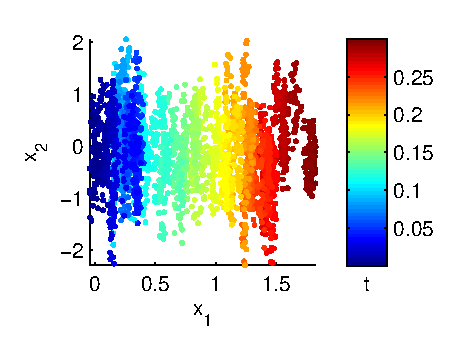
\includegraphics[width=0.35\textwidth]{data_init}};
\node[right=of a](b) {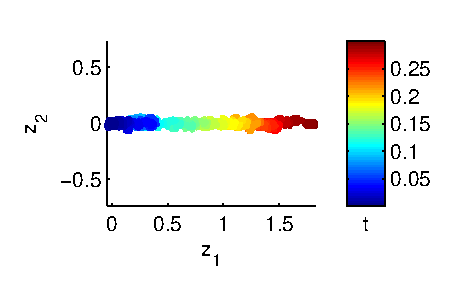
\includegraphics[width=0.35\textwidth]{data_rescaled}};

\draw[->] (a) -- (b);
\end{tikzpicture}

\end{block}

\centering
We will focus on {\bf data reduction}

\end{frame}

%\begin{frame}{Outline}
%
%\tableofcontents
%%\begin{itemize}
%%\item Multiscale SDE framework
%%\item Data reduction (diffusion maps)
%%\item Mahalnobis distance to capture relevant timescales
%%\item Examples
%%\item Conclusion/applications/future work
%%\end{itemize}
%
%\end{frame}

\begin{frame}{Assumed Model for Multiscale Data}


\begin{tikzpicture}

\node[fill=orange!20](a) {$\begin{aligned}
dx_i(t) &= a_i(\vec{x}(t)) dt + dW_i(t), & \: 1 \le i \le m \\
dx_j(t) &= \frac{a_j(\vec{x}(t))}{\epsilon} dt + \frac{1}{\sqrt{\epsilon}} dW_j(t) , & \: m+1 \le j \le n
\end{aligned}$};

\node[below=0.5cm of a, text width=0.5\textwidth,fill=yellow!20, align=center](text1){small parameter $\epsilon$ creates separation of timescales};
\node[above right=0.2cm and -1cm of a, text width=3cm,fill=yellow!20](text2){$m$ slow variables};

\node[below right=0.2cm and -1.5cm of a, text width=3.5cm,fill=yellow!20](text3){$n-m$ fast~variables};


\draw[<-] (-2,-0.75)--(text1);
\draw[<-] (0,-0.75)--(text1);

\draw[<-] (4,0.8)--(text2.south);
\draw[<-] (4,-0.75)--(text3.north);


\end{tikzpicture}

\vspace{0.5cm}
Under some mild conditions, can write a {\em reduced} SDE 

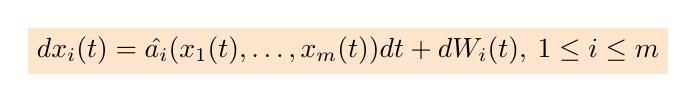
\begin{tikzpicture}

\node[fill=orange!20](a) {$dx_i(t) = \hat{a_i}(x_1(t), \dots, x_m(t)) dt + dW_i(t), \: 1 \le i \le m $};

\end{tikzpicture}

Want to extract a parameterization of $x_1, \dots, x_m$ from {\em data}

\end{frame}


\begin{frame}{Data-Driven Reduction for Multiscale Data}

\centering
{\small Direction of largest variance is not necessarily the {\em slow} direction}

\begin{tikzpicture}
\node(a){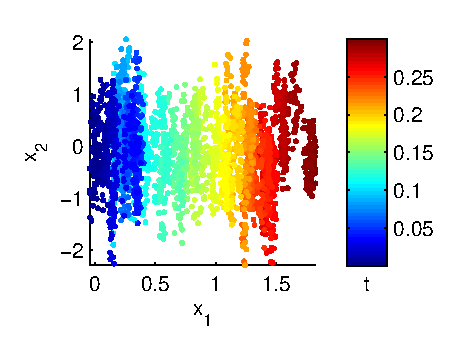
\includegraphics[width=6cm]{data_init}};
\draw[->, red] (-2,-2.25) -- (1,-2.25) node [draw=none,midway,below=0cm, red] {Slow direction};
\draw[->, red] (-3.5,-2) -- (-3.5,2) node [draw=none,midway,left=0cm, rotate=90,red, anchor=center, align=center] {Fast direction\\ Large variance};
\end{tikzpicture}
%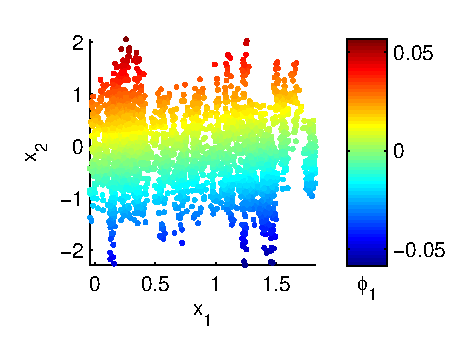
\includegraphics[width=0.5\textwidth]{data_linear_DMAPS}

Construct a {\em metric} which captures relative time scales 

\end{frame}

\begin{frame}{Mahalanobis Distance: A Good Metric}

\centering
The Mahalanobis distance is the Euclidean distance in a rescaled space where each term has unit variance

\begin{block}{Mahalanobis distance, $\| \cdot \|_M$}
$$\| \vec{x}(t_2) - \vec{x}(t_1) \|^2_M = \| \vec{z}(t_2) - \vec{z}(t_1) \|^2_2$$
where $\vec{z}$ obey the following SDEs
$$dz_i(t) = b_i(\vec{z}(t)) dt + dW_i(t)$$
\end{block}

\end{frame}

\begin{frame}{Mahalanobis Distance: A Good Metric}


\centering
For the multiscale SDE we are considering,

\begin{tikzpicture}

\node[fill=orange!20](a) {$\begin{aligned}
dx_i(t) &= a_i(\vec{x}(t)) dt + dW_i(t), & \: 1 \le i \le m \\
dx_i(t) &= \frac{a_i(\vec{x}(t))}{\epsilon} dt + \frac{1}{\sqrt{\epsilon}} dW_i(t) , & \: m+1 \le i \le n
\end{aligned}$};

\node[below=3cm of a,fill=orange!20](b) {$dz_i(t) = b_i(\vec{z}(t)) dt + dW_i(t)$};

\node[align=center,below right=0.5cm and -4.5cm of a, fill=yellow!20](c) {Rescale $x_{m+1}, \dots, x_n$  by $\sqrt{\epsilon}$ \\{\scriptsize $\begin{aligned}
z_i &= x_i, & \: 1 \le i \le m \\
z_i &= \sqrt{\epsilon}x_i , & \: m+1 \le i \le n
\end{aligned}$ \par}};

\draw[fill=orange] (-4,-2.5) ellipse (0.5cm and 1.5cm);
\draw[fill=orange] (-1.5,-2.5) ellipse (0.5cm and 0.5cm);
\draw[->, gray] (-4,-2.5) -- (-4,-1) node[ midway, black] {{\scriptsize $x_2$}};
\draw[->, gray] (-4,-2.5) -- (-3.5,-2.5) node[ midway, black] {{\scriptsize $x_1$}};

\draw[->, gray] (-1.5,-2.5) -- (-1.5,-2) node[ midway, black] {{\scriptsize $z_2$}};
\draw[->, gray] (-1.5,-2.5) -- (-1,-2.5) node[ midway, black] {{\scriptsize $z_1$}};

\path[->, thick] (-3.4,-2.5) edge [bend right] (-2.1,-2.5);

\draw[->](a) -- (b);

\end{tikzpicture}

\end{frame}

\begin{frame}{Mahalanobis Distance Collapses Fast Directions}

\begin{tikzpicture}
\node[fill=orange!20](a) {{\small $\begin{aligned} 
\| \vec{x}(t_2) - \vec{x}(t_1) \|^2_M  &= \| \vec{z}(t_2) - \vec{z}(t_1) \|^2_2 \\
&= \sum_{i=1}^n \left( z_i(t_2) - z_i(t_1) \right)^2 \\
&= \sum_{i=1}^m  \left( x_i(t_2) - x_i(t_1) \right)^2 + \underbrace{\sum_{i=m+1}^n \epsilon \left( x_i(t_2) - x_i(t_1) \right)^2}
\end{aligned}$}};

\node[align=center,below left=0.2cm and -5cm of a, fill=yellow!20](c) {{\scriptsize $\begin{aligned}
z_i &= x_i, & \: 1 \le i \le m \\
z_i &= \sqrt{\epsilon}x_i , & \: m+1 \le i \le n
\end{aligned}$}};

\node[align=center,below right=1cm and -5cm of a, fill=yellow!20, text width=4cm](d) {Fast variables are scaled by $\epsilon$!};

\draw[->](c.north) -- (-2.5,-1.1);
\draw[->](d.north) -- (3.75,-1.75);

\end{tikzpicture}

\end{frame}


\begin{frame}{Nonlinear Data}

\centering
\begin{block}

We could have data
$$\vec{y} = \mathbf{f}(\vec{x})$$
where $\mathbf{f}$ is some nonlinear measurement function
\end{block}

\newfootnote{Coifman and Singer, ACHA, 2009}

\vspace{0.5cm}
Mahalanobis distance is invariant (to fourth order) \\to nonlinear transformations

\begin{block}{}
$\| \vec{y}(t_2) - \vec{y}(t_1) \|^2_M = \| \vec{z}(t_2) - \vec{z}(t_1) \|^2_2 + \mathcal{O}(\|  \vec{y}(t_2) - \vec{y}(t_1) \|^4_2)$
\end{block}

Diffusion maps uses a kernel

Choose kernel width $\sigma_{kernel}$ where errors are small
	
\end{frame}

\begin{frame}{Recap: General Setup}


\begin{itemize}

\item Data $\vec{y}(t_1), \vec{y}(t_2), \dots, \vec{y}(t_N)$


\item $\vec{y} = \mathbf{f}(\vec{x})$, where $\mathbf{f}$ is some nonlinear function


\item $\vec{x}$ comes from a multiscale SDE


\item $\vec{z}$ is $\vec{x}$ rescaled to collapse fast directions



\end{itemize}

\centering
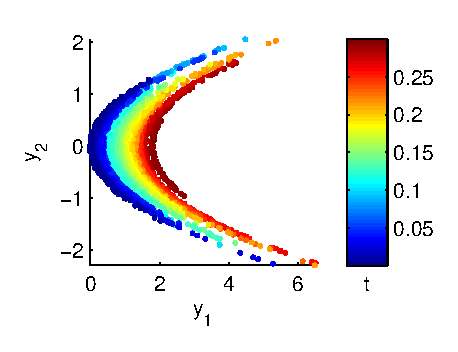
\includegraphics[width=0.3\textwidth]{data_init_nonlinear}
\hfill
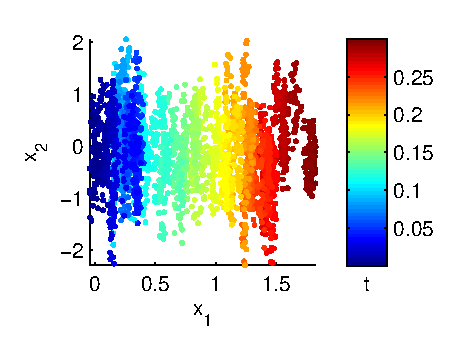
\includegraphics[width=0.3\textwidth]{data_init}
\hfill
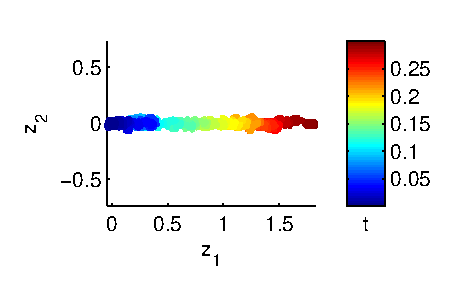
\includegraphics[width=0.3\textwidth]{data_rescaled}

 Want a parameterization of data \\which is one-to-one with the {\em slow variables}

\end{frame}

\begin{frame}{Mahalanobis Distance Approximation}

\centering

 
For diffusion maps,
$W_{ij} = \exp \left( -\frac{\| \vec{z}(t_i) - \vec{z}(t_j) \|_2^2}{\sigma_{kernel}^2} \right) $

Approximate $\| \vec{z}(t_i) - \vec{z}(t_j) \|_2$ using Mahalanobis distance

\vspace{0.5cm}

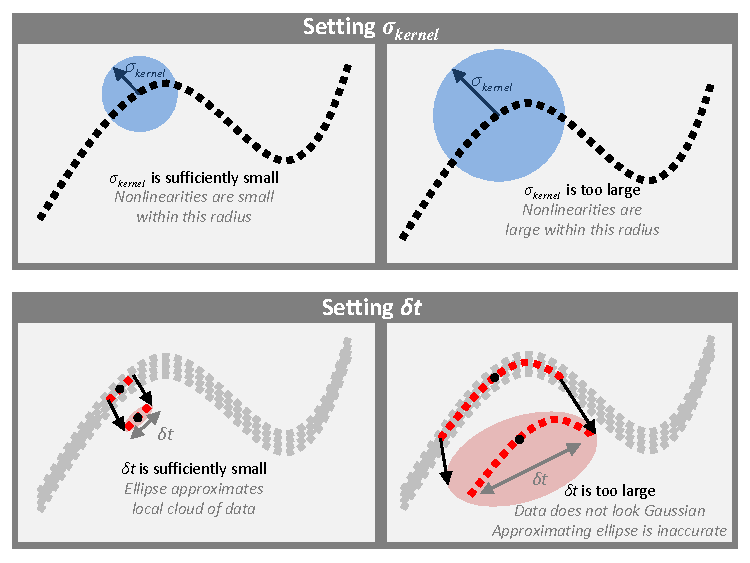
\includegraphics[width=0.8\textwidth, trim=0cm 5cm 0cm 0cm, clip]{schematic}

Choose $\sigma_{kernel}$ such that Mahalanobis distance approximation \\ is accurate
within ball of radius $\sigma_{kernel}$

\end{frame}

\begin{frame}{Errors in Mahalanobis Distance}

Want to write $\| \vec{z}(t_2) - \vec{z}(t_1) \|$ in terms of $\vec{y}(t_1), \vec{y}(t_2)$

\vspace{0.5cm}

By Taylor expansion,
%
\makebox[\textwidth][c]{
\begin{tikzpicture}
\node[fill=orange!20](a) { {\scriptsize $
\begin{aligned}
\| \vec{z}(t_2) - \vec{z}(t_1) \|^2_2 =&
\overbrace{\frac{1}{2} \left(\vec{y}(t_2)-\vec{y}(t_1)\right)^T \left(C^\dagger (\vec{y}(t_1)) + C^\dagger (\vec{y}(t_2)) \right) (\vec{y}(t_2)-\vec{y}(t_1))} \\
&+ \underbrace{ E_M \left(\vec{y}(t_1), \vec{y}(t_2) \right)} + \underbrace{ \mathcal{O} \left(\| \vec{y}(t_2) - \vec{y}(t_1) \|^6_2 \right)}
\end{aligned}
$}};

\node[above=0.5cm of a, fill=yellow!20, align=center, text width=6cm](text1){{\small Mahalanobis distance\\$C$ is the covariance of $\vec{y}$ \\$\dagger$ denotes the pseudoinverse \par}};

\node[below left=0.5cm and -6cm of a, fill=yellow!20, align=center, text width=6cm](text2){{\small $\mathcal{O} \left(\| \vec{y}(t_2) - \vec{y}(t_1) \|^4_2 \right)$ error term\\ Involves second- and higher-order derivatives of $\mathbf{f}^{-1}$ \par}};

\node[below right=0.5cm and -4cm of a, fill=yellow!20, align=center, text width=4cm](text3){{\small Higher-order error term}};


\draw[->] (text1.south) -- (1.1,0.8);
\draw[->] (text2.north) -- (-1.2,-0.8);
\draw[->] (text3.north) -- (1.6,-0.8);

\end{tikzpicture}
}

%\begin{equation}
%\begin{aligned} 
%E_M\left( \vec{y}(t_1), \vec{y}(t_2) \right)
% =
%\frac{1}{2} \sum_{i=1}^n \sum_{jkl=1}^{d} &
%\left( g_{i, (j)} (\vec{y}(t_1)) g_{i, (k,l)} (\vec{y}(t_1)) -  g_{i, (j)} (\vec{y}(t_2)) g_{i, (k,l)} (\vec{y}(t_2)) \right) \\
%& (\vec{y}_j(t_2) - \vec{y}_j(t_1))   (\vec{y}_k(t_2) - \vec{y}_k(t_1))(\vec{y}_l(t_2) - \vec{y}_l(t_1)) \\
%+ \frac{1}{8} \sum_{i=1}^n \sum_{jklm=1}^d  &
%\left( g_{i, (j,k)} (\vec{y}(t_1)) g_{i, (l,m)} (\vec{y}(t_1)) +  g_{i, (j,k)} (\vec{y}(t_2)) g_{i, (l,m)} (\vec{y}(t_2)) \right) \\
%&(\vec{y}_j(t_2) - \vec{y}_j(t_1))  (\vec{y}_k(t_2) - \vec{y}_k(t_1))(\vec{y}_l(t_2) - \vec{y}_l(t_1)) (\vec{y}_m(t_2) - \vec{y}_m(t_1)) \\
%+ \frac{1}{6} \sum_{i=1}^n \sum_{jklm=1}^d &
%\left( g_{i, (j)} (\vec{y}(t_1)) g_{i, (k,l,m)} (\vec{y}(t_1)) +  g_{i, (j)} (\vec{y}(t_2)) g_{i, (k,l,m)} (\vec{y}(t_2)) \right) \\
%& (\vec{y}_j(t_2) - \vec{y}_j(t_1))  (\vec{y}_k(t_2) - \vec{y}_k(t_1))(\vec{y}_l(t_2) - \vec{y}_l(t_1))(\vec{y}_m(t_2) - \vec{y}_m(t_1))
%\end{aligned}
%\end{equation}
%%
%where
%%
%\begin{equation}
%\begin{aligned}
%g_{i,(j)} &= \sqrt{e_i} \frac{\partial g_i}{\partial y_j}
%\\
%g_{i,(j,k)} &= \sqrt{e_i}  \frac{\partial^2 g_i}{\partial y_j \partial y_k}
%\\
%g_{i,(j,k,l)} &= \sqrt{e_i}  \frac{\partial^3 g_i}{\partial y_j \partial y_k \partial y_l}
%\end{aligned}
%\end{equation}

\end{frame}

\begin{frame}{Setting the Kernel Scale}

\centering
{\small  
For diffusion maps,
$W_{ij} = \exp \left( -\frac{\| \vec{z}(t_i) - \vec{z}(t_j) \|_2^2}{\sigma_{kernel}^2} \right) $


Choose $\sigma_{kernel}$ where Mahalanobis distance $\sim \| \vec{z}(t_i) - \vec{z}(t_j) \|_2$
}

\begin{tikzpicture}
\node[fill=orange!20](a) { {\scriptsize $
\begin{aligned}
\| \vec{z}(t_2) - \vec{z}(t_1) \|^2_2 =&
{ \color{blue} \frac{1}{2} \left(\vec{y}(t_2)-\vec{y}(t_1)\right)^T \left(C^\dagger (\vec{y}(t_1)) + C^\dagger (\vec{y}(t_2)) \right) (\vec{y}(t_2)-\vec{y}(t_1))} \\
&+ {\color{red} E_M \left(\vec{y}(t_1), \vec{y}(t_2) \right)} + { \mathcal{O} \left(\| \vec{y}(t_2) - \vec{y}(t_1) \|^6_2 \right)}
\end{aligned}
$}};

\node[below=0cm of a](b){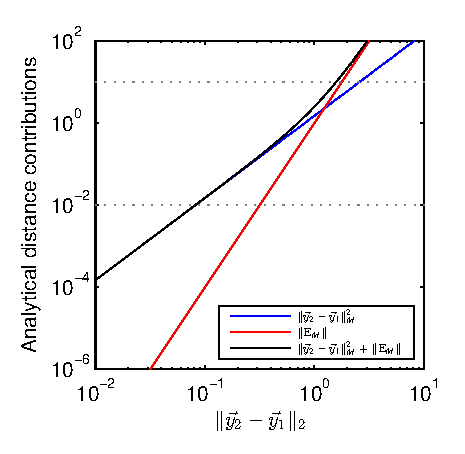
\includegraphics[width=0.5\textwidth]{dist_dy_analytical_nonlinear}};

\node[right=0.5cm of b, text width=4cm](text1){{\scriptsize Mahalanobis distance dominates\par}};
\node[above right=-1cm and 0.5cm of b, text width=4cm](text2){{\scriptsize Errors dominate \par}};

\draw[->] (text1.west) -- (2.5,-3.25);
\draw[->] (text2.west) -- (2.5,-1.65);

\draw[fill=yellow, opacity=0.2] (-1.7, -5.25) rectangle (2.4, -2);

\node[left=0cm of b, align=center, text width=2.2cm](text3){{\scriptsize Acceptable range  for $\sigma_{kernel}$ \par}};
\draw[->] (text3) -- (-1.5, -3);

\end{tikzpicture}

\end{frame}

\begin{frame}{Setting the Kernel Scale Empirically}

\begin{tikzpicture}
%\node[fill=orange!20](a) { {\scriptsize $
%\begin{aligned}
%\| \vec{z}(t_2) - \vec{z}(t_1) \|^2_2 =&
%{\frac{1}{2} \left(\vec{y}(t_2)-\vec{y}(t_1)\right)^T \left(C^\dagger (\vec{y}(t_1)) + C^\dagger (\vec{y}(t_2)) \right) (\vec{y}(t_2)-\vec{y}(t_1))} \\
%&+ { E_M \left(\vec{y}(t_1), \vec{y}(t_2) \right)} + { \mathcal{O} \left(\| \vec{y}(t_2) - \vec{y}(t_1) \|^6_2 \right)}
%\end{aligned}
%$}};

\node[fill=orange!20](a) { {\small Choose kernel scale $\sigma_{kernel}$ where $\| \vec{y}_2 - \vec{y}_1 \|^2_M \propto \| \vec{y}_2 - \vec{y}_1 \|^2_2$
}};

\node[below=0.25cm of a](b){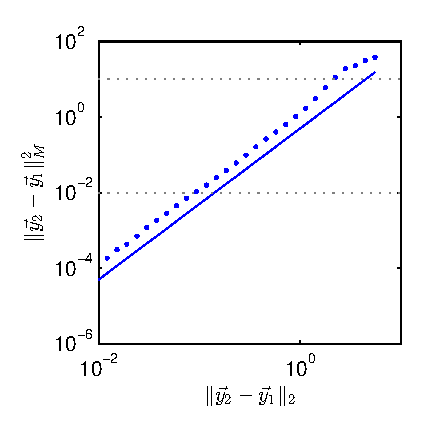
\includegraphics[width=0.5\textwidth]{dist_dy_nonlinear}};

\node[right=0.5cm of b, text width=4cm](text1){{\scriptsize Mahalanobis distance dominates\par}};
\node[above right=-1cm and 0.5cm of b, text width=4cm](text2){{\scriptsize Errors dominate \par}};

\draw[->] (text1.west) -- (2.5,-3.25);
\draw[->] (text2.west) -- (2.5,-1.65);

\draw[fill=yellow, opacity=0.2] (-1.55, -5.25) rectangle (2.6, -2);

\end{tikzpicture}

\centering

\end{frame}

\begin{frame}{Calculating the Mahalanobis Distance}

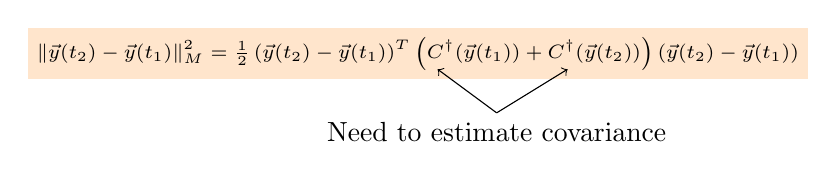
\begin{tikzpicture}

\node[fill=orange!20]{{\scriptsize 
$\| \vec{y}(t_2) - \vec{y}(t_1) \|^2_M =
\frac{1}{2} \left(\vec{y}(t_2)-\vec{y}(t_1)\right)^T \left(C^\dagger (\vec{y}(t_1)) + C^\dagger (\vec{y}(t_2)) \right) (\vec{y}(t_2)-\vec{y}(t_1)) $ \par}};

\node (a) at (1,-1)  {Need to estimate covariance};
\draw[->] (a.north) -- (1.9,-0.2);
\draw[->] (a.north) -- (0.25,-0.2);
\end{tikzpicture}

\vspace{0.5cm}

\centering
Estimate using simulation bursts of length $\delta t$
%{\scriptsize
%$$\hat{C}_{ij} (\vec{x}_t, \delta t)
%=
%{\frac{1}{\delta t} \left( \mathbb{E} \left[ y_i (t+\delta t) y_j (t+ \delta t) \mid \vec{y}(t) \right]
%- \mathbb{E} \left[ y_i (t+\delta t) \mid \vec{y}(t) \right] \mathbb{E} \left[ y_j (t+\delta t) \mid \vec{y}(t) \right] \right)}$$
%}

\begin{tikzpicture}
\node(a) {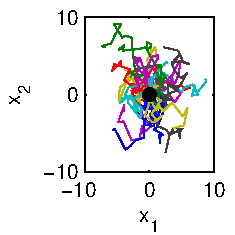
\includegraphics[width=0.3\textwidth]{mahalanobis_trajectories}};
\node[right=0.25cm of a](b) {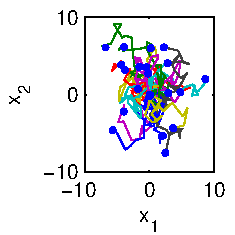
\includegraphics[width=0.3\textwidth]{mahalanobis_trajectories2}};
\node[right=0.25cm of b](c) {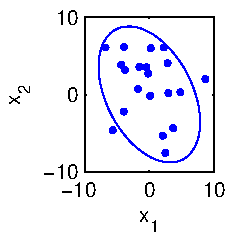
\includegraphics[width=0.3\textwidth]{mahalanobis_points2}};

\node[below right=0cm and -3.25cm of a, text width=0.3\textwidth, align=center](texta) {{\scriptsize Run many simulations of length $\delta t$ starting from initial point \par}};
\node[below right=0cm and -3.25cm of b, text width=0.3\textwidth, align=center](textb) {{\scriptsize Collect cloud of final points \par}};
\node[below right=0cm and -3.25cm of c, text width=0.3\textwidth, align=center](textc) {{\scriptsize Fit ellipse \par}};

\end{tikzpicture}

\end{frame}

\begin{frame}{Covariance Estimation}

\centering

 
Estimate local covariance by fitting an ellipse to data

\vspace{0.5cm}

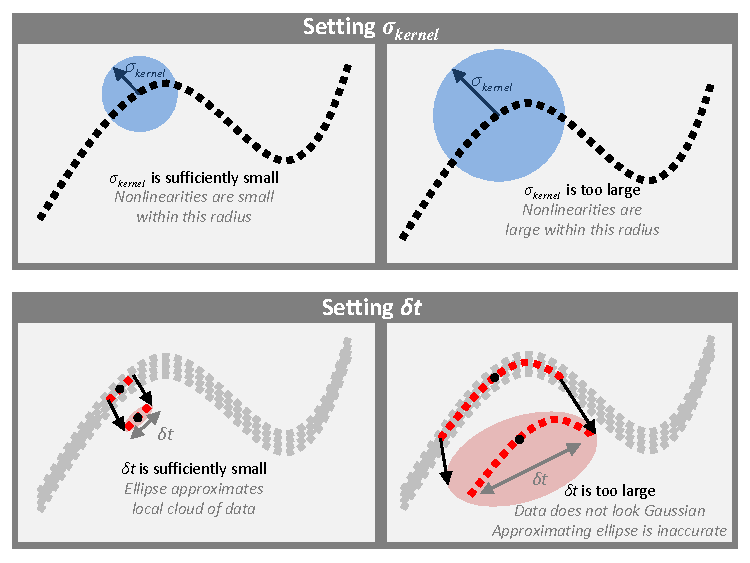
\includegraphics[width=\textwidth, trim=0cm 0cm 0cm 5cm, clip]{schematic}

\vspace{0.5cm}

Choose $\delta t$ such that nonlinear effects are minimal 

\end{frame}



\begin{frame}{Errors from covariance estimation}

By It\={o}-Taylor expansion of $\mathbf{f}$ and $\vec{x}(t)$,

\makebox[\textwidth][c]{
\begin{tikzpicture}
\node[fill=orange!20](a) { {\scriptsize $
\begin{aligned}
\hat{C}_{ij} (\vec{x}_t, \delta t)
=&
\overbrace{\frac{1}{\delta t} \left( \mathbb{E} \left[ y_i (t+\delta t) y_j (t+ \delta t) \mid \vec{y}(t) \right]
- \mathbb{E} \left[ y_i (t+\delta t) \mid \vec{y}(t) \right] \mathbb{E} \left[ y_j (t+\delta t) \mid \vec{y}(t) \right] \right)}
\\
=& \underbrace{\sum_{k=1}^m \left. \frac{\partial f_{i}}{\partial x_k} \right|_{\vec{x}(t)} \left. \frac{\partial f_{j}}{\partial x_k} \right|_{\vec{x}(t)}
+ \frac{1}{\sqrt{\epsilon}} \sum_{k=m+1}^n  \left. \frac{\partial f_{i}}{\partial x_k} \right|_{\vec{x}(t)} \left. \frac{\partial f_{j}}{\partial x_k} \right|_{\vec{x}(t)}}
+ \underbrace{E_{C, ij} (\vec{x}(t), \delta t)} + \underbrace{\mathcal{O}(\delta t^{3/2})}
\end{aligned}
$}};

\node[above=0.5cm of a, fill=yellow!20, align=center, text width=6cm](text1){{\small Empirically estimate local covariance \par}};

\node[below left=0.5cm and -3cm of a, fill=yellow!20, align=center, text width=3cm](text2){{\small True covariance \par}};

\node[below=0.5cm of a, fill=yellow!20, align=center, text width=4cm](text3){{\small $\mathcal{O} (\delta t)$ error term \\ Depends on drift, and second- and higher-order derivatives of $\mathbf{f}$  \par}};

\node[below right=0.5cm and -3cm of a, fill=yellow!20, align=center, text width=3	cm](text4){{\small $\mathcal{O} (\delta t^{3/2})$ error term}};

\draw[->] (text1.south) -- (0.6,1.1);
\draw[->] (text2.north) -- (-0.9,-1.1);
\draw[->] (text3.north) -- (3.5,-0.8);
\draw[->] (text4.north) -- (5.25,-0.8);

\end{tikzpicture}
}

%\begin{equation}\label{eq:estimated_cov}
%\begin{aligned}
%\hat{C}_{ij} (\vec{x}_t, \delta t)
%=&
%\frac{1}{\delta t} \left( \mathbb{E} \left[ y_i (t+\delta t) y_j (t+ \delta t) \mid \vec{y}(t) \right]
%- \mathbb{E} \left[ y_i (t+\delta t) \mid \vec{y}(t) \right] \mathbb{E} \left[ y_j (t+\delta t) \mid \vec{y}(t) \right] \right)
%\\
%=& \sum_{k=1}^n \frac{1}{e_k} \left. \frac{\partial f_{i}}{\partial x_k} \right|_{\vec{x}(t)} \left. \frac{\partial f_{j}}{\partial x_k} \right|_{\vec{x}(t)}
%+ E_{C, ij} (\vec{x}(t), \delta t) + \mathcal{O}(\delta t^{3/2})
%%=& \sum_{k=1}^n \frac{1}{e_k} \left. \frac{\partial f_{i}}{\partial x_k} \right|_{\vec{x}(t)} \left. \frac{\partial f_{j}}{\partial x_k} \right|_{\vec{x}(t)} \\
%%&+ \frac{1}{\delta t} \sum_{k=1}^n f_{i,(k)}(\vec{x}(t)) \left( \mathbb{E} \left[ \int_t^{t+\delta t} \int_{s_1}^{t+\delta t} f_{j,(k,0)}(\vec{x}(s_2)) ds_2 ds_1 \right]
%%+ \mathbb{E} \left[  \int_t^{t+\delta t} \int_t^{s_2} f_{j,(0,k)}(\vec{x}(s_1)) ds_1 ds_2\right] \right) \\
%%&+  \frac{1}{\delta t} \sum_{k=1}^n f_{j,(k)}(\vec{x}(t)) \left( \mathbb{E} \left[ \int_t^{t+\delta t} \int_{s_1}^{t + \delta t} f_{i,(k,0)}(\vec{x}(s_2)) ds_2 ds_1 \right]
%%+ \mathbb{E} \left[ \int_t^{t+\delta t} \int_t^{s_2} f_{i,(0,k)}(\vec{x}(s_1)) ds_1 ds_2 \right] \right) \\
%%&+  \frac{1}{\delta t} \sum_{k,l=1}^n \mathbb{E} \left[ \int_t^{t+\delta t}\left( \int_t^{s_2} f_{i,(k,l)}(\vec{x}(s_1)) dW_{s_1, k}  \right) \left(  \int_t^{s_2} f_{j,(k,l)}(\vec{x}(s_1)) dW_{s_1, k} \right) ds_2 \right] \\
%%&+ \mathcal{O} (\delta t^{3/2}),
%\end{aligned}
%\end{equation}
%%
%where $E_C = \mathcal{O} (\delta t)$ is an error term, with
%%
%\begin{equation} \label{eq:cov_error}
%\begin{aligned}
%E_{C, ij} (\vec{x}(t), \delta t) =&
% \frac{1}{\delta t} \sum_{k=1}^n f_{i,(k)}(\vec{x}(t)) \mathbb{E} \left[ \int_t^{t+\delta t} \left( \int_{s_2}^{t+\delta t} f_{j,(k,0)}(\vec{x}(s_1)) ds_1
%+ \int_t^{s_2} f_{j,(0,k)}(\vec{x}(s_1)) ds_1 \right) ds_2 \right] \\
%&+  \frac{1}{\delta t} \sum_{k=1}^n f_{j,(k)}(\vec{x}(t))  \mathbb{E} \left[ \int_t^{t+\delta t} \left( \int_{s_2}^{t + \delta t} f_{i,(k,0)}(\vec{x}(s_1)) ds_1
%+  \int_t^{s_2} f_{i,(0,k)}(\vec{x}(s_1)) ds_1 \right) ds_2 \right] \\
%&+  \frac{1}{\delta t} \sum_{k,l=1}^n \mathbb{E} \left[ \int_t^{t+\delta t}\left( \int_t^{s_2} f_{i,(k,l)}(\vec{x}(s_1)) dW_{s_1, k}  \right) \left(  \int_t^{s_2} f_{j,(k,l)}(\vec{x}(s_1)) dW_{s_1, k} \right) ds_2 \right]
%\end{aligned}
%\end{equation}

\end{frame}

\begin{frame}{Setting the Covariance Timescale}

\makebox[\textwidth][c]{
\begin{tikzpicture}
\node[fill=orange!20](a) { {\scriptsize $
\hat{C}_{ij} (\vec{x}_t, \delta t)
= {\color{blue} \sum_{k=1}^m \left. \frac{\partial f_{i}}{\partial x_k} \right|_{\vec{x}(t)} \left. \frac{\partial f_{j}}{\partial x_k} \right|_{\vec{x}(t)}
+ \frac{1}{\sqrt{\epsilon}} \sum_{k=m+1}^n  \left. \frac{\partial f_{i}}{\partial x_k} \right|_{\vec{x}(t)} \left. \frac{\partial f_{j}}{\partial x_k} \right|_{\vec{x}(t)}}
+ { \color{red} E_{C, ij} (\vec{x}(t), \delta t)} + {\mathcal{O}(\delta t^{3/2})}
$}};

\node[below=1cm of a](b){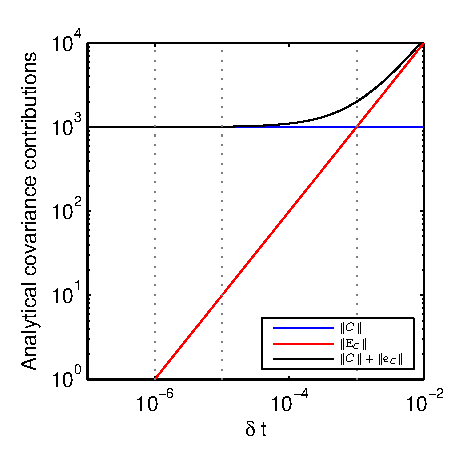
\includegraphics[width=0.5\textwidth]{C_dt_analytical_linear}};

\node[above left=0.25cm and -2cm of b](text1){True covariance dominates};
\node[right=3cm of text1](text2){Errors dominate};

\draw[->] (text1.south) --  (-1,-1.8);
\draw[->] (text1.south) --  (-0.1,-1.8);
\draw[->] (text2.south) --  (1.5,-1.8);

\draw[fill=yellow, opacity=0.2] (-1.8, -6.1) rectangle (1.5, -1.9);

\node[below=0cm of b](text3){{\scriptsize Acceptable range of $\delta t$}};

\draw[->] (text3.north) --  (0,-6.0);

\end{tikzpicture}
}

\end{frame}

\begin{frame}{Setting the Covariance Timescale Empirically}

\makebox[\textwidth][c]{
\begin{tikzpicture}
\node[fill=orange!20](a) { {\small Find where $\hat{C}$ is constant with respect to $\delta t$
}};

\node[below=1cm of a](b){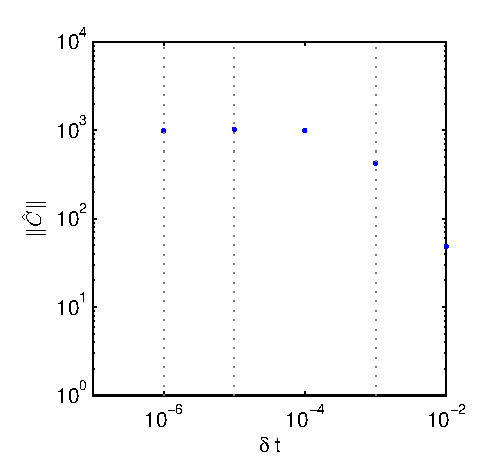
\includegraphics[width=0.5\textwidth]{C_dt_linear}};

\node[above left=0.25cm and -2cm of b](text1){True covariance dominates};
\node[right=3cm of text1](text2){Errors dominate};

\draw[->] (text1.south) --  (-1,-1.8);
\draw[->] (text1.south) --  (-0.1,-1.8);
\draw[->] (text2.south) --  (1.5,-1.8);

\draw[fill=yellow, opacity=0.2] (-1.8, -6) rectangle (1.5, -1.8);

\node[below=0cm of b](text3){{\small Acceptable range of $\delta t$}};

\draw[->] (text3.north) --  (0,-6.0);


\end{tikzpicture}
}


\end{frame}


\begin{frame}{Linear Two-Dimensional Data}

\begin{block}{}	
\begin{equation*} 
\begin{aligned}
dx_1(t) &=& adt &+& dW_1(t)\\
dx_2(t) &=& -\frac{x_2(t)}{\epsilon} dt &+& \frac{1}{\sqrt{\epsilon}} dW_2(t)
\end{aligned}
\end{equation*} 
\end{block}

\centering
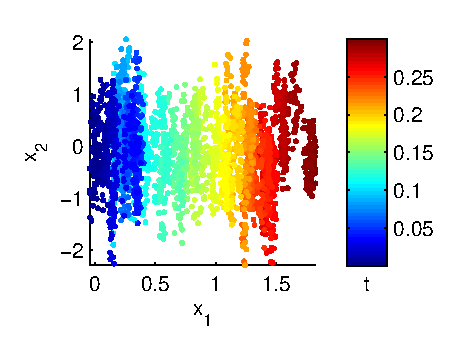
\includegraphics[width=0.45\textwidth]{data_init}

$x_1$ is the slow variable, $x_2$ is the fast variable \newfootnote{$a=3$, $\epsilon = 10^{-3}$}

\end{frame}

\begin{frame}{Reduction of Linear Data}

\begin{tikzpicture}
\node<.(2)->(a){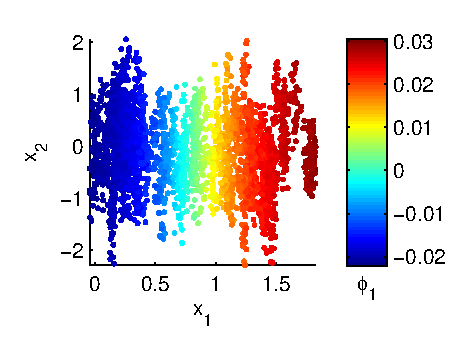
\includegraphics[width=0.5\textwidth]{data_linear_NIV}};
\node[left=0cm of a](b){ 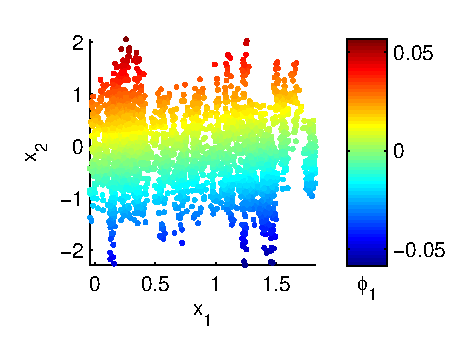
\includegraphics[width=0.5\textwidth]{data_linear_DMAPS}};

\node<.(2)->[above=0cm of a, text width=0.45\textwidth, align=center](texta1){Using Mahalanobis distance};
\node<.(2)->[below=0cm of a, text width=0.4\textwidth, align=center](texta2){{\scriptsize Parameterization is consistent with slow variable $x_1$ \par}};

\node[above=0cm of b, text width=0.4\textwidth, align=center](textb1){Using Euclidean distance};
\node[below=0cm of b, text width=0.4\textwidth, align=center](textb2){{\scriptsize Parameterization is inconsistent with slow variable $x_1$ \par}};

\node<.(2)->[below=of a](c){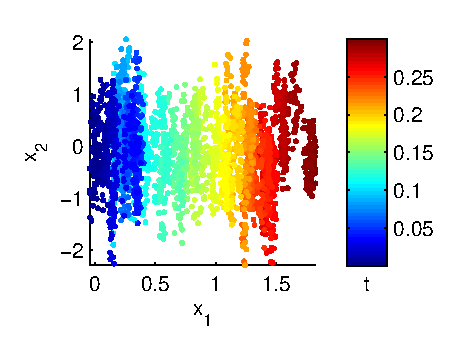
\includegraphics[width=0.2\textwidth]{data_init}};
\node<.(2)->[left=0cm of c]{{\scriptsize Data colored by time}};

\end{tikzpicture}

\end{frame}

\begin{frame}{Curved ``Half-Moon'' Data}

\begin{block}{}
\begin{equation*}
\begin{aligned}
dx_1(t) =& adt + dW_1(t)\\
dx_2(t) =& -\frac{x_2(t)}{\epsilon} dt + \frac{1}{\sqrt{\epsilon}} dW_2(t)\\
\begin{bmatrix}
y_1(t) \\ y_2(t)
\end{bmatrix} =&
\mathbf{f}(\vec{x}(t)) =
\begin{bmatrix}
x_1(t) + x_2^2(t) \\
x_2(t)
\end{bmatrix}
\end{aligned}
\end{equation*}
\end{block}

\centering
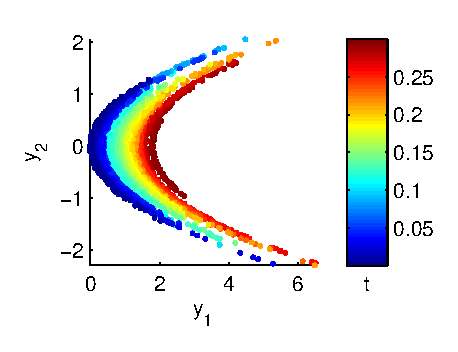
\includegraphics[width=0.5\textwidth]{data_init_nonlinear}

\end{frame}


\begin{frame}{Reduction of Nonlinear Data}

\begin{tikzpicture}

\node(a){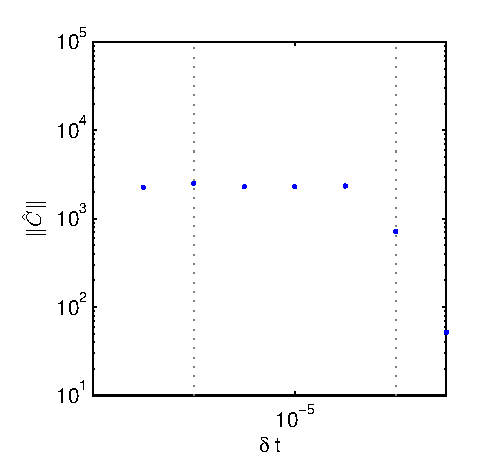
\includegraphics[width=0.3\textwidth]{C_dt_nonlinear}};
\node[below=0cm of a](b){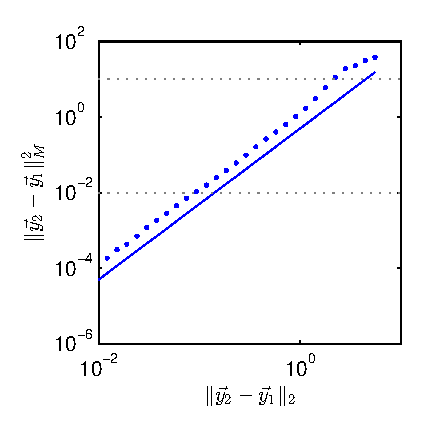
\includegraphics[width=0.3\textwidth]{dist_dy_nonlinear}};

\node[below right=-3cm and 1cm of a, align=center, text width=0.5\textwidth](c){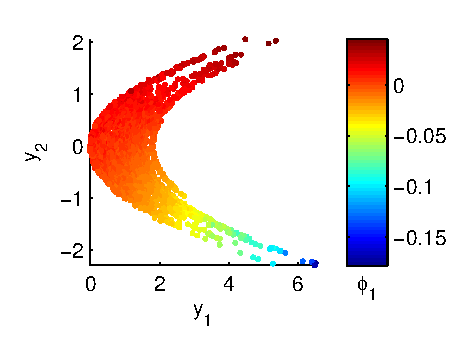
\includegraphics[width=\textwidth]{data_nonlinear_NIV_dt2_kernel1} \\ $\delta t$ is too large \\ {\scriptsize Parameterization is not \\ one-to-one with slow variable \par}};

\draw[->, red] (1.15, 1.7) -- (1.15,1.45);
\draw[->, red] (1.85, -3.35) -- (1.6,-3.35);

\end{tikzpicture}

\end{frame}

\begin{frame}{Reduction of Nonlinear Data}

\begin{tikzpicture}

\node(a){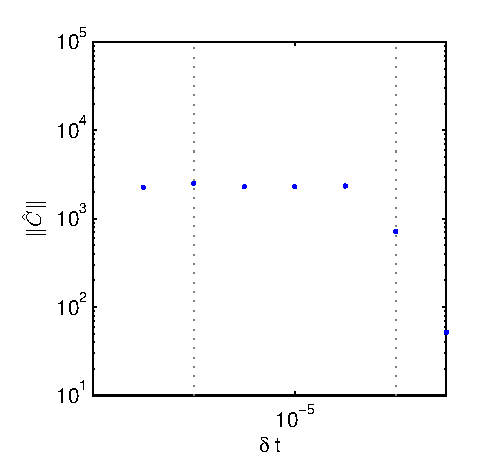
\includegraphics[width=0.3\textwidth]{C_dt_nonlinear}};
\node[below=0cm of a](b){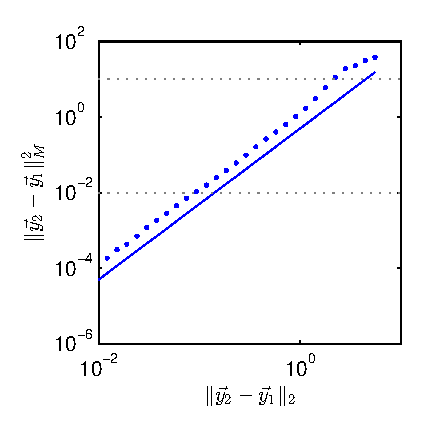
\includegraphics[width=0.3\textwidth]{dist_dy_nonlinear}};

\node[below right=-3cm and 1cm of a, align=center, text width=0.5\textwidth](c){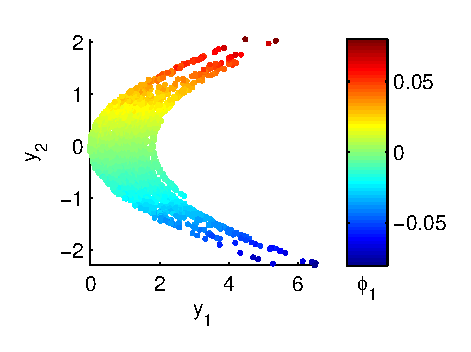
\includegraphics[width=\textwidth]{data_nonlinear_NIV_dt1_kernel2} \\  $\sigma_{kernel}$ is too large \\{\scriptsize Parameterization is not \\ one-to-one with slow variable \par}};

\draw[->, red] (-0.35, 1.7) -- (-0.35,1.45);
\draw[->, red] (1.85, -2.4) -- (1.6,-2.4);

\end{tikzpicture}

\end{frame}

\begin{frame}{Reduction of Nonlinear Data}

\begin{tikzpicture}

\node(a){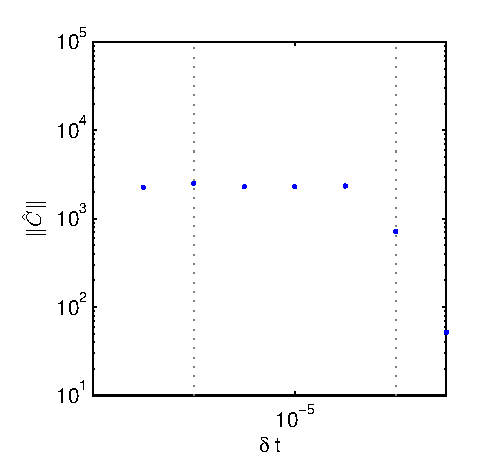
\includegraphics[width=0.3\textwidth]{C_dt_nonlinear}};
\node[below=0cm of a](b){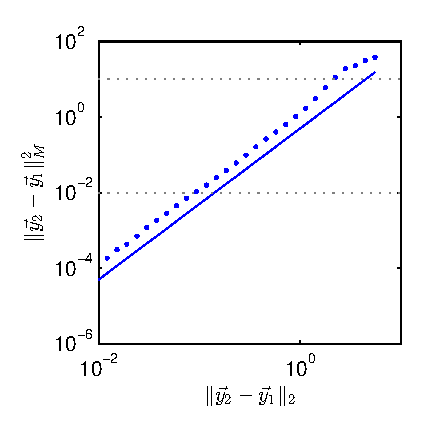
\includegraphics[width=0.3\textwidth]{dist_dy_nonlinear}};

\node[below right=-3cm and 1cm of a, align=center, text width=0.5\textwidth](c){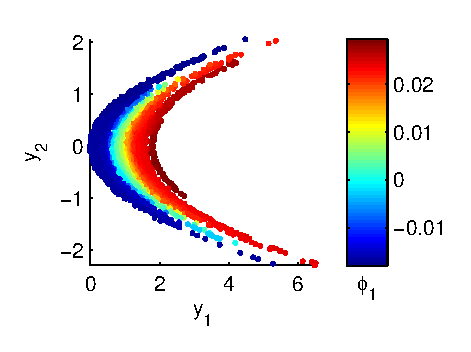
\includegraphics[width=\textwidth]{data_nonlinear_NIV_dt1_kernel1} \\ Using an appropriate value of $\delta t$ and $\sigma_{kernel}$ \\ {\scriptsize Parameterization is \\ one-to-one with slow variable \par}};

\draw[->, red] (-0.35, 1.7) -- (-0.35,1.45);
\draw[->, red] (1.85, -3.35) -- (1.6,-3.35);

\end{tikzpicture}

\end{frame}


\begin{frame}{Data from Molecular Dynamics Simulations}

	Simulate alanine dipeptide (Ala2) in explicit solvent \\
	{\tiny AMBER 10 molecular simulation package;
    optimized version of the AMBER ff03 force field;
    TIP3P water molecules;
    periodic boundary conditions;
    particle mesh Ewald method for long-range electrostatic interactions;
    NVT ensemble;
    temperature being maintained at 300~K with a Langevin thermostat;
    hydrogen bond lengths are fixed using the SHAKE algorithm \par}
    
    \begin{minipage}[t]{0.5\textwidth}
        \centering
        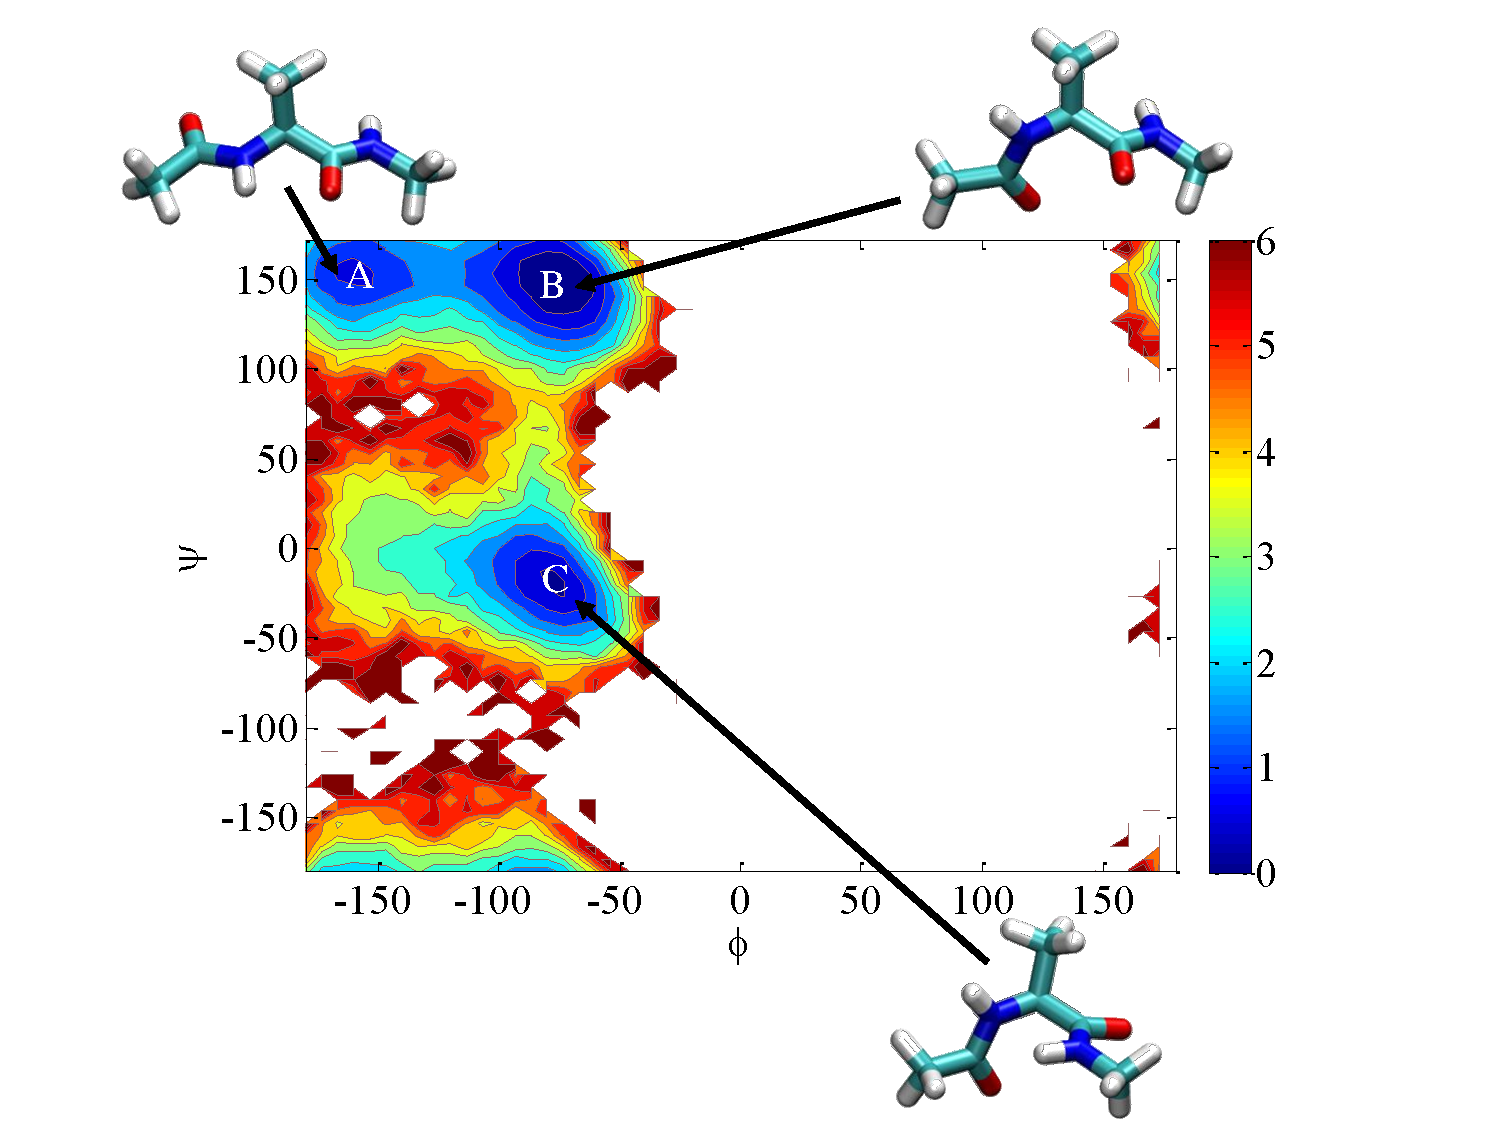
\includegraphics[width=\textwidth]{FES}\\
        {\small The free energy surface (FES) of Ala2 has three distinct wells}
    \end{minipage}
    \hfill
    \begin{minipage}[t]{0.4\textwidth}
        \centering
        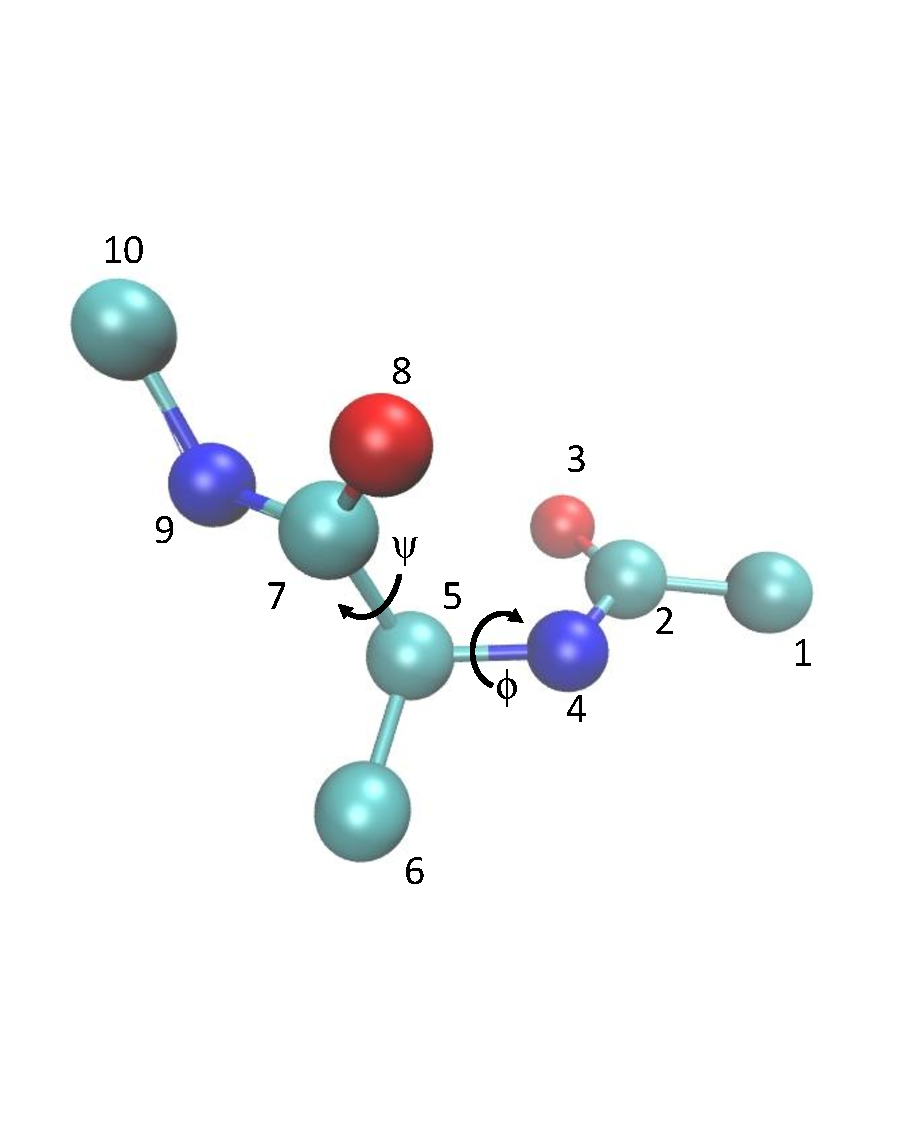
\includegraphics[width=0.6\textwidth]{molecule2}\\
        {\small The FES is well parameterized by the two dihedral angles $\phi$ and $\psi$}
    \end{minipage}

    \vspace{0.1in}
    We collect data around well B in the free energy surface

\end{frame}

\begin{frame}{Diffusion Maps Embeddings}

	{\small
	Mahalanobis distance factors out nonlinear measurement functions \\
	Different measurements yield consistent embeddings
	\par}
	
    \begin{minipage}[t]{0.45\textwidth}
        \centering
        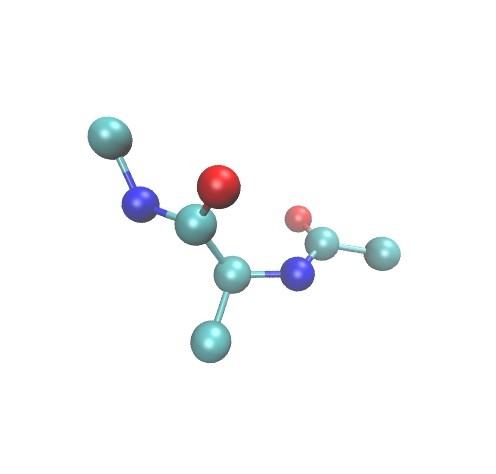
\includegraphics[width=0.5\textwidth, trim=0in 0.2in 0in 0.2in, clip]{molecule_all}\\
        {\scriptsize In one data set, we observe all the atoms in the molecule \par}
    \end{minipage}
    \hfill
    \begin{minipage}[t]{0.45\textwidth}
        \centering
        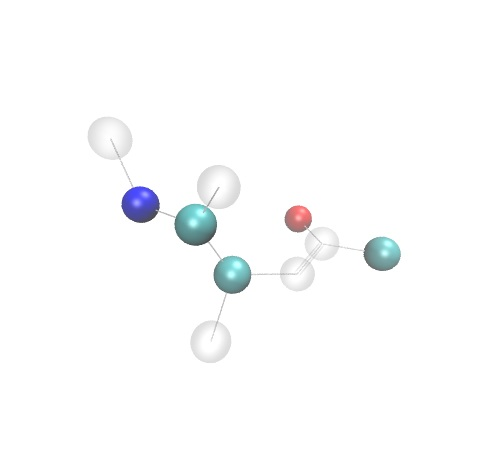
\includegraphics[width=0.5\textwidth, trim=0in 0.2in 0in 0.2in, clip]{molecule_odd}\\
        {\scriptsize In one data set, we observe {\em only} the odd atoms in the molecule \par}
    \end{minipage}

    \vspace{0.2in}

    \centering
    {\scriptsize 
    \begin{minipage}{0.2\textwidth}
        \centering
        \includegraphics[width=\textwidth]{ala2_embed1}\\
        (a)
    \end{minipage}
%    \hfill
    \begin{minipage}{0.2\textwidth}
        \centering
        \includegraphics[width=\textwidth]{ala2_embed2}\\
        (b)
    \end{minipage}
%    \hfill
    \begin{minipage}{0.2\textwidth}
        \centering
        \includegraphics[width=\textwidth]{ala2_embed3}\\
        (c)
    \end{minipage}}
    
    \vspace{0.1in}
        {\small We obtain (visually) consistent embeddings for the two data sets }

    {\em \scriptsize The 3-dimensional NIV embeddings for Ala2 colored by (a) the y-coordinate of the first atom, (b) the dihedral angle $\phi$, and (c) the dihedral angle $\psi$. \par}

\end{frame}

\begin{frame}{Reconstructions of Molecular Configurations}
	
		\makebox[\textwidth][c]{

	\begin{tikzpicture}
	
	\node(a) {\includegraphics[width=2cm]{ala2_embed1}};
	\node[right=3cm of a](b) {\includegraphics[width=2cm, trim=0in 0.2in 0in 0.2in, clip]{molecule_all}};
	
	\draw[->] (a.east) -- (b.west) node[above, midway, text width=3.5cm, align=center] {{\scriptsize Train function \\ $h:$ embedding $\mapsto$ atoms \par}};
	
	\node[below=0.1cm of a](d){\includegraphics[width=2cm]{ala2_embed1}};
	
	\node[left=2cm of d](c){\includegraphics[width=2cm, trim=0in 0.2in 0in 0.2in, clip]{molecule_odd}};
	\node[right=3cm of d](e) {\includegraphics[width=2cm, trim=0in 0.2in 0in 0.2in, clip]{molecule_all}};
	
	\draw[->] (c.east) -- (d.west) node[above, midway, text width=3.5cm, align=center] {{\scriptsize Calculate embedding of odd atoms \par}};
	\draw[->] (d.east) -- (e.west) node[above, midway, text width=3.5cm, align=center] {{\scriptsize Calculate locations of all atoms using $h$\par}};

	\node[below=0cm of d](molec1){\includegraphics[width=0.25\textwidth,trim=0in 5in 0in 0in, clip]{molecule300_balls}};
	\node[right=0cm of molec1](molec2){\includegraphics[width=0.25\textwidth,trim=0in 5in 0in 0in, clip]{molecule600_balls}};
	\node[left=0cm of molec1](molec3){\includegraphics[width=0.25\textwidth,trim=0in 5in 0in 0in, clip]{molecule900_balls}};
	
	\node[below=-0.2cm of molec1, align=center, text width=0.75\textwidth](molec_text){{\scriptsize \em True structure (black) and reconstructed structure (red) for three different data points \par}};
	
	\draw[fill=gray, opacity=0.2] (molec3.north west) rectangle (molec_text.south east);
	
	%\includegraphics[width=0.25\textwidth,trim=0in 5in 0in 0in, clip]{molecule600_balls}
	%\includegraphics[width=0.25\textwidth,trim=0in 5in 0in 0in, clip]{molecule900_balls}%\\
	%{\scriptsize \em True structure (black) and reconstructed structure (red) for three different data points}
	%};
	
	\end{tikzpicture}
	}

\end{frame}

\begin{frame}{Conclusions}

\begin{itemize}
\item Multiscale stochastic data arises in a variety of contexts
\item Adapt data mining techniques to incorporate time scales
\item Extract slow variables from nonlinear data
\item Future work: using extracted slow variables \\to write reduced models

\end{itemize}

\vspace{2cm}
\centering
\includegraphics[width=4cm]{csgf_logo}
\hspace{2cm}
\includegraphics[width=2cm]{nsf_logo}

\end{frame}

\section{Developmental Dynamics}

\begin{frame}{Reconstructing Dynamics from Snapshots}

Two types of data collection schemes% \\ when studying developmental dynamics

\begin{description}
\item[Longitudinal] Developmental trajectory of {\em a single organism} \\is monitored over time
\item[Cross-sectional] Samples from {\em many organisms} are collected; each organism contributes only a single snapshot from the developmental process
\end{description}

%\vspace{0.1in}
\begin{center}
We will look at cross-sectional imaging data. %The tasks are
%then to \textcolor{bold}{register} and \textcolor{bold}{temporally order} the snapshots to obtain a representative developmental trajectory.

\includegraphics[width=2in]{fig1}

{\scriptsize A caricature of ordering cross-sectional data. \\
(Left) Fish, each in a different stage of development.  (Right) Fish, now registered and temporally ordered. \par}
\end{center}

\end{frame}

\begin{frame}{Dynamics of {\em Drosophila} Embryogenesis}

\begin{minipage}[b]{0.7\textwidth}
{\small
 {\em Drosophila melanogaster} (common fruit fly): model organism in developmental biology \par}
%
\end{minipage}
\hspace{0.2in}
\includegraphics[width=0.7in]{drosophila_picture}

\begin{center}
We will look at optical sections \\ perpendicular to the long axis of the embryo

\includegraphics[width=2.5in]{drosophila_schematic}

\begin{tikzpicture}
\node[] (a) {\includegraphics[width=1.25in]{longitudinal_45min}};
\node[right=0.4in of a] (b) {\includegraphics[width=0.75in]{DV_45min}};
\draw[->] (a.east) -- (b.west);
\end{tikzpicture}

\end{center}

\end{frame}

\begin{frame}{Data Collection}

\begin{center}
\includegraphics[width=4in]{drosophila_imaging_setup}

\vspace{0.2in}

We obtain images at a fixed depth (90~$\mu m$) \\from the tip of the embryo.

Each embryo is in a different rotational orientation.

\end{center}

\newfootnote{Chung {\em et al}, {\em Nature Methods}, 2011}

\end{frame}

\begin{frame}{A Typical Data Set}
\begin{center}
\includegraphics[width=0.75\textwidth]{drosophila_data_unordered}
\end{center}


\begin{itemize}
{\small
\item Each image is from a different embryo 
\item Each embryo is stained for three different proteins
\item Each embryo is at a different (and unknown) developmental time
\item Each embryo is also at a different (and unknown) orientation
\par}
\end{itemize}


\end{frame}

\begin{frame}{Methods for Registration and Ordering}

\centering
Simultaneously register and order using vector diffusion maps 
\newfootnote{Singer and Wu, Commun Pure Appl Math, 2012}

\includegraphics[width=0.6\textwidth]{synchronization_schematic}

\end{frame}

\begin{frame}{Registered and Ordered Images}

\centering 

Compared vector diffusion maps ordering \\
with manual ordering by an expert

\includegraphics[width=0.7\textwidth]{drosophila_data_ordered}
%
\includegraphics[width=0.25\textwidth]{drosophila_data_corr}

Can compute an {\em average developmental trajectory}
\includegraphics[width=\textwidth]{drosophila_data_averaged}

\end{frame}

\begin{frame}{Conclusions}

\end{frame}

\section{Detecting the true dimensionality}

\begin{frame}{Detecting the dimensionality of data}

In PCA, we look at the eigenvalues

In DMAPS, also look at eigenvalues -- but there is an issue

\end{frame}

\begin{frame}{Repeated eigendirections}

\includegraphics[width=1in]{strip_discrete1}
\includegraphics[width=1in]{strip_discrete2}
\includegraphics[width=1in]{strip_discrete3}
\includegraphics[width=1in]{strip_discrete4}

\end{frame}

\begin{frame}{Algorithm: local linear regression}

Fit a function $\phi_k = f(\phi_1, \dots, \phi_{k-1})$. 

If fit is accurate, then $\phi_k$ is a {\em repeated eigendirection}

If fit is inaccurate, then $\phi_k$ is a {\em unique eigendirection}


\end{frame}

\begin{frame}{Example: swiss roll}

\end{frame}

\begin{frame}{Application: Chemotaxis}

\end{frame}

\begin{frame}{Results}

\end{frame}

\begin{frame}{Conclusions}

\end{frame}


\end{document}

